\chapter{Introduction}
\label{chap:intro}

The main objective of the work presented in this thesis is the measurement of CP violation in the decay \BstoJpsiphi. This measurement is a
test of the current model of elementary-particle interactions. It is performed within the LHCb experiment, which studies particles produced
in the proton--proton collisions of the Large Hadron Collider (LHC) at \cern{} in Geneva, Switzerland. The results presented here (see also
reference~\cite{LHCb-PAPER-2014,LHCb-ANA-2014-039}) are an update of previous LHCb results \cite{LHCb-PAPER-2013-002,*LHCb-ANA-2012-067}
with a dataset that is more than three times larger.

Motivations for such a test of particle-physics models are discussed in Section~\ref{sec:intro_SM}. The measurement is introduced in
Sections~\ref{sec:intro_Jpsiphi} and \ref{sec:intro_LHCb}, after an introduction to CP violation in this context in
Section~\ref{sec:intro_CPV}.

Details of the phenomenology of the \BstoJpsiphi{} decay are discussed in Chapter~\ref{chap:pheno}. A discussion of the measurement and
the applied data-analysis techniques can be found in Chapter~\ref{chap:ana}. Finally, results of the measurement are presented in
Chapter~\ref{chap:result}.

\section{The Standard Model of Particle Physics}
\label{sec:intro_SM}

%%%%%%%%%%%%%%%%%%%%%%%%%%%%%%%%%%%%%%%%%%%%%
\subsection{Elementary-Particle Interactions}
\label{subsec:intro_SM_int}
%%%%%%%%%%%%%%%%%%%%%%%%%%%%%%%%%%%%%%%%%%%%%

Interactions between quarks and leptons are described by the \emph{Standard Model of particle physics} (Standard Model, SM). The Standard
Model unifies the electromagnetic and weak forces in a theory of \emph{electroweak
interactions}~\cite{Glashow:1961tr,*Weinberg:1967tq,*Salam:1968rm}, while strong interactions are described separately by \emph{Quantum
Chromodynamics} (QCD)~\cite{Fritzsch:1973pi}. Both theories are based on quantum field theory, in which quarks and leptons are described as
fermionic fields that interact via bosonic fields.

In the electroweak model there are four vector bosons that mediate interactions, three of which acquire a mass through the
\emph{Brout-Englert-Higgs} (BEH) \emph{mechanism}~\cite{Englert:1964et,*Higgs:1964ia,*Higgs:1964pj,*Guralnik:1964eu}. Generating particle
masses with this mechanism implies the existence of the scalar \emph{Higgs boson}, which was recently discovered by the \atlas{} and
CMS experiments at the LHC~\cite{Aad:2012tfa,*Chatrchyan:2012ufa}. The BEH mechanism is believed to be also responsible for generating the
masses of quarks and leptons through so-called Yukawa interactions.

The three massive vector bosons are the $\Wp$, the $\Wm$ and the $\Zz$. These particles are the carriers of the weak interaction. The
remaining massless vector boson is the photon, which mediates the electromagnetic interaction.

Contrary to leptons, quarks carry the ``charge'' of the strong force, or \emph{colour}. This makes them subject to strong interactions,
described by QCD. The mediators of the strong interaction are gluons, which come in eight different types and are themselves colour-charged
particles.

One of the features of the strong force is that it becomes weaker with increasing interaction energy. This phenomenon is called
\emph{asymptotic freedom}~\cite{Gross:1973id,*Politzer:1973fx}. The increasing interaction strength with decreasing energy (or,
equivalently, increasing interaction distance) makes it impossible to completely separate coloured particles. As a result, quarks and
gluons are \emph{confined} within colour-neutral objects, such as hadrons.

%Whenever possible, \emph{perturbation theory} is used to do calculations of particle interactions. Amplitudes for interaction processes are
%expanded as a series in powers of the coupling strength of the interaction. If the coupling strength is small, the exact solution of the
%calculation can be approximated by the leading terms in the series. In QCD this only works for high-energy processes, where the strong
%force is weak. For low-energy QCD processes, like interactions between quarks inside hadrons, the series diverges and non-perturbative
%methods have to be applied.
%
%\begin{table}[hbt]
%  \begin{tabular}{rccc}
%    \hline
%                      &  1st generation         &  2nd generation    &  3rd generation    \\
%    \hline
%    down-type quarks  &  down (d)               &  strange (s)       &  beauty (b)        \\
%    up-type quarks    &  up (u)                 &  charm (c)         &  top (t)           \\
%    charged leptons   &  electron ($\lepe[-]$)  &  muon ($\lmu[-]$)  &  tau ($\ltau[-]$)  \\
%    neutrinos         &  $\nue$                 &  $\numu$           &  $\nutau$          \\
%    \hline
%  \end{tabular}
%  \caption{Quarks and leptons.}
%  \label{tab:quarksLeptons}
%\end{table}
%Both quarks and leptons come in different \emph{flavours}, which are ordered in three generations. This structure is shown in
%Table~\ref{tab:quarksLeptons}. Strong, electromagnetic, and the neutral (Z$^0$) weak interactions conserve flavour and work within a
%generation. In the Standard Model, the only interaction that changes the flavour of quarks and leptons is the charged (W$^\pm$) weak
%interaction \cite{Cabibbo:1963yz,Glashow:1970gm,Kobayashi:1973fv,Pontecorvo:1957cp,*Pontecorvo:1957qd,*Maki:1962mu,*Pontecorvo:1967fh}.
%Mixing of quark flavours is discussed in more detail in Section~\ref{subsec:intro_mixCPV_mix}.

Low-energy QCD interactions between quarks and gluons within hadrons are so strong that they cannot be described with \emph{perturbation
theory}, where amplitudes are expanded as a series in the coupling strength of the interaction. The series would diverge and the exact
solution of a calculation is not approximated by the leading terms in the series. Numerical methods may be applied to treat low-energy
QCD interactions in an alternative way. Strong interactions at high energies and electroweak interactions can be described with
perturbative methods.

Decays of hadrons that contain heavy quarks can be approximately described using a \emph{factorization} approach. In the case of $\Bs$
mesons, for example, the decay of the constituent b quark is treated separately from the strong interactions among the quarks in the $\Bs$
meson and its decay products. The decay takes place at a relatively high energy scale set by the b-quark mass and is calculated
perturbatively. The strong hadronic interactions are less energetic and non-perturbative.

For the decay of a (heavy) quark or lepton a transition to one of the lighter quarks or leptons is required. In the Standard Model, such a
\emph{flavour change} is only possible in a weak interaction that is mediated by the $\Wpm$
boson~\cite{Cabibbo:1963yz,Glashow:1970gm,Kobayashi:1973fv}. This mixing of quark flavours in the context of meson decays is discussed in
more detail in Section~\ref{subsec:intro_mixCPV_mix}.

%For each particle in the Standard Model there is also an antiparticle. Particle and antiparticle states are related by the \emph{charge
%conjugation} operation (C). Since the weak interaction couples to left-handed particle states and right-handed antiparticle states, an
%additional operation is needed to obtain the equivalent antimatter interactions. This operation, which inverts spatial coordinates, is a
%\emph{parity transformation} (P).

Another interesting property of the weak interaction is that it only couples to left-handed particle states and to right-handed
antiparticle states. As a result, two transformations are needed to obtain the equivalent antiparticle interaction for a given particle
interaction: A \emph{charge-conjugation} operation (C) transforms particles into the corresponding antiparticles and a \emph{parity}
operation (P) inverts spatial coordinates, which transforms left-handed states into right-handed states.

Most interactions in the Standard Model are invariant under the combined C and P operation, which makes matter and antimatter almost
symmetric. The only source of CP-symmetry violation is the flavour-changing weak interaction. Measurements of the amount of CP violation
provide tests of the Standard Model description of particle interactions, which is discussed in Section~\ref{subsec:intro_mixCPV_CPV}.

In addition to the charge and parity operations there is the transformation of \emph{time reversal} (T), which inverts the time coordinate.
Quantum field theory is based on the principle of Lorentz invariance, which implies invariance under a combined C, P, and T transformation
for any interaction. CPT is assumed to be an exact symmetry in the studies presented in this thesis.


%%%%%%%%%%%%%%%%%%%%%%%%%%%%%%%%%%%%%%
\subsection{Beyond the Standard Model}
\label{subsec:intro_SM_beyond}
%%%%%%%%%%%%%%%%%%%%%%%%%%%%%%%%%%%%%%

Since the start of its construction in the 1960s, the Standard Model has been tested extensively by experiments. Elementary-particle
interactions have been studied over a wide range of energies, with particles from different sources. The Standard Model has proven to be
a consistent description of particle physics.

Despite its success, there are strong motivations for developing descriptions of particle physics that go beyond the Standard Model. Some
of these motivations are theoretical, while others are based on experimental observations.

The Standard Model contains 18 parameters, for which it predicts no values. There are nine unpredicted quark and lepton masses, the mass
and vacuum expectation value of the Higgs field, four quark-mixing parameters (see Section~\ref{subsec:intro_mixCPV_mix}), and three
interaction coupling constants. These parameters have been measured, but it would be more satisfying to have a more fundamental description
without unpredicted quantities.

Another missing feature in the Standard Model is unification of all forces. While the electric and magnetic forces are unified in
electromagnetism and the electromagnetic and weak forces in electroweak theory, the Standard Model does not attempt to unify the
electroweak and strong forces. The gravitational force is left out completely. Although not strictly necessary to describe current
particle-physics experiments, the knowledge of how to describe all these phenomena consistently would significantly improve our
understanding of nature.

There is a more practical theoretical issue known as the \emph{hierarchy problem}. The mass of the Higgs boson is affected by quantum
corrections from loops of other particles. These corrections are large and with only the particles in the Standard Model one would expect
the Higgs mass to be much larger than the measured value~\cite{Weinberg:1975gm,*Susskind:1978ms,*'tHooft:1979bj}. The only way to get
around this within the Standard Model is a careful fine-tuning of its parameters, which is considered to be unnatural.

Several experimental observations also indicate that the current Standard Model is incomplete. Experiments studying neutrinos from various
sources have observed transitions between neutrinos from different
generations~\cite{Fukuda:1998mi,*Ahmad:2002jz,*Eguchi:2002dm,*An:2012eh}. This implies mixing between leptons of different flavours, but
also non-zero neutrino masses. Neutrinos are massless in the original Standard Model, but in principle their masses can be included by a
minimal extension, assuming neutrino masses have the same origin as quark and charged-lepton masses.

There is also a more exciting possibility to include neutrino masses. Since all quantum numbers of neutrinos and antineutrinos are equal,
neutrinos may be their own antiparticles, which could lead to Majorana mass components~\cite{Majorana:1937vz}. This scenario would open up
new possibilities to explain why neutrino masses are so much smaller than quark and charged-lepton masses. The masses of the left-handed
Standard Model neutrinos could be suppressed by the very large masses of hypothetical right-handed Majorana neutrinos via a so-called
\emph{see-saw mechanism} \cite{Minkowski:1977sc}.

A related observation is that the universe contains matter, but almost no antimatter. One of the required conditions to create such an
imbalance is a sufficient amount of CP violation in particle interactions~\cite{Sakharov:1967dj}. CP violation in the Standard Model is
believed to be too small to generate the large matter--antimatter asymmetry that is
observed~\cite{Gavela:1993ts,*Huet:1994jb,*Gavela:1994dt}.

The right-handed neutrinos introduced by a see-saw mechanism would also provide a natural way to introduce the required additional CP
violation in particle interactions. Couplings of charged leptons to these neutrinos would in general be CP violating, which leads to a
lepton--antilepton asymmetry in neutrino decays. This asymmetry for leptons could subsequently lead to an asymmetry for
baryons~\cite{Kuzmin:1985mm,*Fukugita:1986hr}.

Also other cosmological observations suggest the need for extensions of the Standard Model. If measurements of the spatial fluctuations in
the cosmic microwave background are interpreted with the current cosmological models, the bulk of the matter in the universe has an unknown
origin~\cite{Hinshaw:2012aka}. Less than a fifth is conventional matter, which consists of Standard Model particles. The remainder does not
interact strongly or electromagnetically and is therefore termed \emph{dark matter}. The Standard Model does not provide any particles that
would be viable candidates to form dark matter.

Besides see-saw mechanisms, there are many other ideas how to extend the Standard Model, or even to find a more fundamental theory. A
popular candidate is \emph{Supersymmetry}~\cite{Golfand:1971iw,*Volkov:1973ix,*Wess:1974tw}, which leads to a class of models to be tested
by experiments. Supersymmetry is based on an additional symmetry between bosons and fermions, which would give all particles in the
Standard Model a so called ``superpartner''. Introducing these additional particles could solve the hierarchy problem, may provide a
dark-matter candidate, and could be a first step towards unification of the electroweak and strong forces. See reference
\cite{Feng:2013pwa} for a recent review of the status of Supersymmetry.

To make progress in the search for a more complete theory, observations of particle interactions that cannot be described with the Standard
Model are needed. There are two different approaches to search for such inconsistencies. One can assume a particular beyond-the-Standard
Model theory and test its predictions in a measurement. An example of this \emph{top-down} approach is to search for signs of the
additional particles predicted by Supersymmetry. The other method is a \emph{bottom-up} search, where the Standard Model predictions are
tested instead.

In the bottom-up approach one generally searches for small deviations in predictions for well-known processes. An example is the work
presented here, which is a study of the variables in the decay of a Standard Model particle, the $\Bs$ meson. This particle is produced
abundantly in the proton--proton collisions of the LHC and its decays have been studied previously by other collider experiments. One of
the particularly interesting decays is that into a $\Jpsi$ and a $\phimes$ meson, which could exhibit CP
violation~\cite{Nir:1990hj,*Silverman:1998uj,*Ball:1999yi,*Dunietz:2000cr}.

CP violation in the \BstoJpsiphi{} decay%
\footnote{The symbol ``$\phimesalt$'' will be understood to mean ``$\phimes$'' in this context.}
as predicted by the Standard Model is very small. Studies of various extensions of the Standard Model show that it can be significantly
enhanced by introducing new contributions to this process~\cite{Buras:2009if,Chiang:2009ev,*Datta:2009fk}. The decay is also experimentally
accessible, which makes it an excellent tool to search for deviations from the Standard Model prediction.

The $\Bs$ meson and the \BstoJpsiphi{} decay will be further introduced in Section~\ref{sec:intro_Jpsiphi}. First an overview of CP
violation within the context of the Standard Model is given in the next section.

\section{Quark-Flavour Physics and CP Violation}
\label{sec:intro_CPV}

%%%%%%%%%%%%%%%%%%%%%%%%%%%%%%%
\subsection{Quark Mixing}
\label{subsec:intro_mixCPV_mix}
%%%%%%%%%%%%%%%%%%%%%%%%%%%%%%%

The Feynman diagrams for the charged weak current that changes the flavour of a quark are shown in Figure~\ref{fig:WCouplings}. The
subscript ``L'' on the quark indicates that only quark states with a left-handed chirality participate in this interaction.
\begin{figure}[hbt]
  {\sffamily %%BoundingBox: -1 -1 61 36 
%%HiResBoundingBox: -1 -1 60.7757 35.86916 

\hspace*{0.03\textwidth}
\begin{fmffile}{graphics/intro/WCouplings/up}
  \fmfframe(8,16)(8,16){
    \begin{fmfgraph*}(60,35)
      \fmfstraight
      \fmftop{id,ou}
      \fmfbottom{iW}
      \fmf{fermion}{id,v,ou}
      \fmf{boson}{iW,v}
      \fmflabel{d$_\text{L}^\prime$}{id}
      \fmflabel{u$_\text{L}^{\phantom{\prime}}$}{ou}
      \fmflabel{W}{iW}
    \end{fmfgraph*}
  }
\end{fmffile}
\hfill
\begin{fmffile}{graphics/intro/WCouplings/charm}
  \fmfframe(8,16)(8,16){
    \begin{fmfgraph*}(60,35)
      \fmfstraight
      \fmftop{id,ou}
      \fmfbottom{iW}
      \fmf{fermion}{id,v,ou}
      \fmf{boson}{iW,v}
      \fmflabel{s$_\text{L}^\prime$}{id}
      \fmflabel{c$_\text{L}^{\phantom{\prime}}$}{ou}
      \fmflabel{W}{iW}
    \end{fmfgraph*}
  }
\end{fmffile}
\hfill
\begin{fmffile}{graphics/intro/WCouplings/top}
  \fmfframe(8,16)(8,16){
    \begin{fmfgraph*}(60,35)
      \fmfstraight
      \fmftop{id,ou}
      \fmfbottom{iW}
      \fmf{fermion}{id,v,ou}
      \fmf{boson}{iW,v}
      \fmflabel{b$_\text{L}^\prime$}{id}
      \fmflabel{t$_\text{L}^{\phantom{\prime}}$}{ou}
      \fmflabel{W}{iW}
    \end{fmfgraph*}
  }
\end{fmffile}
\hspace*{0.03\textwidth}
}
  \caption{Charged-current weak interactions of quarks.}
  \label{fig:WCouplings}
\end{figure}

The primes on the d$_\text{L}^\prime$, s$_\text{L}^\prime$ and b$_\text{L}^\prime$ quarks in the figure indicate that the states that
couple to the W boson are not the quark mass eigenstates. The down-type states in the interaction are given by a rotation of the mass
eigenstates, which is parameterized by the Cabibbo-Kobayashi-Maskawa (CKM) quark-mixing matrix \cite{Kobayashi:1973fv}:
\begin{equation}
  \begin{pmatrix} \text{d}_\text{L}^\prime \\ \text{s}_\text{L}^\prime \\ \text{b}_\text{L}^\prime \end{pmatrix}
    \equiv \VCKM\, \begin{pmatrix} \text{d}_\text{L} \\ \text{s}_\text{L} \\ \text{b}_\text{L} \end{pmatrix}
    \equiv \begin{pmatrix} \Vud & \Vus & \Vub \\ \Vcd & \Vcs & \Vcb \\ \Vtd & \Vts & \Vtb \end{pmatrix}
           \begin{pmatrix} \text{d}_\text{L} \\ \text{s}_\text{L} \\ \text{b}_\text{L} \end{pmatrix}
    \ .
\end{equation}
Diagrams with W-boson vertices in which one of the three mass eigenstates is selected are proportional to the appropriate matrix element
$V_{ij}$. A similar mechanism applies for mixing of leptons \cite{Pontecorvo:1957cp,*Pontecorvo:1957qd,*Maki:1962mu,*Pontecorvo:1967fh}.

The CKM matrix is a unitary complex matrix. The number of independent parameters in the matrix is limited by the constraint of unitarity
and by the fact that part of the complex phases of the matrix elements can be absorbed in the arbitrary phases of the quark fields.
Representation of the CKM matrix in terms of the four remaining parameters is convention dependent. A commonly used choice is the
\emph{Wolfenstein parameterization} with real-valued $\Vud$, $\Vus$, $\Vcb$, and $\Vtb$ and a single complex phase entering in the other
elements \cite{Wolfenstein:1983yz,*Chau:1984fp,*Buras:1994ec}. Four real parameters, $\lam$, $A$, $\rho$, and $\eta$, are then
defined by
\begin{equation}
  \begin{gathered}
    \lam \equiv \frac{|\Vus|}{\sqrt{|\Vud|^2 + |\Vus|^2}}
      \quad
      A\lam^2 \equiv \frac{|\Vcb|}{\sqrt{|\Vud|^2 + |\Vus|^2}}
      \quad
      A\lam^3(\rho+i\eta) \equiv \Vub[*]
      \ \ .
  \end{gathered}
\end{equation}

The Wolfenstein parameterization of the CKM matrix is motivated by the orders of magnitude of matrix elements. The magnitudes of the
diagonal elements $\Vud$, $\Vcs$ and $\Vtb$, which describe the coupling between up-type and down-type quarks of the same generation, are
approximately equal to one. Magnitudes of the couplings between the first and second generation are between a factor four and five smaller:
$|\Vus|\approx|\Vcd|\approx\lam\approx0.23$ \cite{Charles:2004jd,Bona:2005vz}.

Couplings between the second and third and between the first and third generation are suppressed by factors $\lam^2$ and $\lam^3$,
respectively: $|\Vcb|\approx|\Vts|\approx A\lam^2\approx0.04$, $|\Vub|=A\lam^3|\rho+i\eta|\approx0.004$, and $|\Vtd|\approx
A\lam^3|1-\rho-i\eta|\approx0.009$. In this form of the Wolfenstein parameterization the complex phase is introduced with the parameters
$\rho\approx0.13$ and $\eta\approx0.36$, where $\arg(\Vub[*])=\arg(\rho+i\eta)\approx70^\circ$.

%Expanding the CKM matrix in terms of the small parameter $\lam$ within the Wolfenstein parameterization yields
%\begin{equation}
%  \begin{split}
%    \VCKM =& \begin{pmatrix}
%               1 - \tfrac{1}{2}\lam^2 - \tfrac{1}{8}\lam^4  &  0  &  0 \\
%               0  &  1 - \tfrac{1}{2}\lam^2 - \tfrac{1}{8}\lam^4 (1+4A^2) & 0 \\
%               0  &  0  &  1 - \tfrac{1}{2}A^2\lam^4
%             \end{pmatrix} \\
%          &+ \phantom{A}\lam\phantom{^2}
%            \begin{pmatrix}
%               \phantom{-}0                                   &  1            &  0     \\
%               -\left[1 - \tfrac{1}{2}A^2\lam^4(1-2r)\right]  &  \quad0\quad  &  \ 0\  \\
%               \phantom{-}0                                   &  0            &  0
%            \end{pmatrix} \\
%          &+ A\lam^2
%            \begin{pmatrix}
%               0     &  0                                             &  0    \\
%               0     &  0                                             &  1    \\
%               \ 0\  &  -\left[ 1 - \tfrac{1}{2}\lam^2(1-2r) \right]  &  \ 0\
%            \end{pmatrix} \\
%          &+ A\lam^3
%            \begin{pmatrix}
%               0                                &  \quad0\quad  &  r^*\  \\
%               0                                &  0            &  0     \\
%               1 - (1 - \tfrac{1}{2}\lam^2)\,r  &  0            &  0
%            \end{pmatrix}
%           + \mathcal{O}(\lam^6)
%    \ .
%  \end{split}
%\end{equation}

The CKM matrix can be expanded in terms of the small parameter $\lam$. Neglecting terms of order $\lam^4$ and higher relative to the
leading term for each element, it is approximated by \cite{Charles:2004jd}
\begin{equation}
  \label{eq:CKMApprox}
  \VCKM \approx
    \begin{pmatrix}
      c                  &  \lam                           &  \!\! A\lam^3\,r^* \\
      -\lam              &  c                              &  A\lam^2           \\
      A\lam^3(1 - c\,r)  &  \!\! -A\lam^2 (c + \lam^2\,r)  &  1
    \end{pmatrix}
    \ ,
\end{equation}
where $c\equiv1 - \tfrac{1}{2}\lam^2$ and $r\equiv\rho+i\eta$.

Notice that only the elements $\Vub$, $\Vtd$ and $\Vts$ have non-vanishing imaginary parts in this approximation. In $\Vts$ the parameter $r$ is suppressed by a
factor $\lam^2$, which makes the imaginary part of this element much smaller than the real part. For $\Vcd$ and $\Vcs$ the suppression
factors are $\lam^4$ and $\lam^6$, respectively, which results in vanishing imaginary parts.


%%%%%%%%%%%%%%%%%%%%%%%%%%%%%%%
\subsection{CP Violation}
\label{subsec:intro_mixCPV_CPV}
%%%%%%%%%%%%%%%%%%%%%%%%%%%%%%%

The Standard Model mixing formalism was introduced for quarks, but it also applies to antiquarks. A CP operation on the states in
Figure~\ref{fig:WCouplings} results in the interactions of right-handed antiquark states with the W boson.

In the transformation from quarks to antiquarks the CKM-matrix elements in the weak interaction states are replaced with their complex
conjugates. If there were no complex phase in the CKM matrix, its elements would be real and the weak interactions of quarks would be
invariant under the CP transformation. Introducing a complex phase breaks this invariance and gives rise to CP violation.

Although the complex phase in the CKM matrix formally breaks CP invariance, CP-violating phenomena cannot be observed directly in processes
that are described by a single diagram with W-boson interactions. The magnitude of a diagram is squared to obtain the corresponding
observable probability, which makes its phase unobservable.

CP violation can only be observed in processes where two or more amplitudes with different CKM elements interfere. The CKM elements then
introduce a different \emph{weak phase} for each contribution, which changes sign between CP-conjugate processes. Differences between the
weak phases do affect the observable magnitude of the total amplitude if the contributing amplitudes also have different \emph{strong
phases}, which do not change sign under a CP transformation.

This can be illustrated by considering two interfering amplitudes $A_1$ and $A_2$ with CKM factors $F_1$ and $F_2$. The asymmetry between
the squared magnitudes for CP-conjugate processes is then given by
\begin{equation}
  \label{eq:interference}
  \begin{split}
    A_\text{CP} &\equiv \frac{|\Af[]|^2 - |\Abarf[]|^2}{|\Af[]|^2 + |\Abarf[]|^2}
                 = \frac{|F_1\,A_1 + F_2\,A_2|^2 - |F_1^*\,A_1 + F_2^*\,A_2|^2}{|F_1\,A_1 + F_2\,A_2|^2 + |F_1^*\,A_1 + F_2^*\,A_2|^2} \\
                &= \frac{-2 R\, \sin(\Delta\delta)\, \sin(\Delta\phi)}{1 + R^2 + 2 R\, \cos(\Delta\delta)\, \cos(\Delta\phi)}
                   \ ,
  \end{split}
\end{equation}
where $R\equiv\frac{|F_2|\,|A_2|}{|F_1|\,|A_1|}$, $\Delta\delta\equiv\arg(A_2)-\arg(A_1)$ and $\Delta\phi\equiv\arg(F_2)-\arg(F_1)$. Notice
that the CP asymmetry vanishes if there is no weak phase difference $\Delta\phi$, but also if there is no strong phase difference
$\Delta\delta$. The size of the asymmetry also depends on the relative magnitudes of the amplitudes and CKM factors. The asymmetry vanishes
in case the $|F_2|\,|A_2|$ is much smaller than $|F_1|\,|A_1|$.

To construct convention-independent measures of CP violation in quark interactions, the CKM-matrix unitarity constraints are used. The
unitarity relation $\VCKM[\dagger]\VCKM = \VCKM\VCKM[\dagger] = \mathbb{1}$ gives nine constraints. Six of these are orthogonality
relations, two of which are given by
\begin{subequations}
  \label{eq:unitConstraints}
  \begin{align}
    \text{d--b:} & \quad \Vud\Vub[*] + \Vcd\Vcb[*] + \Vtd\Vtb[*] = 0 \nonumber \\
    \label{eq:unitConstraints_d}
    &\qquad\qquad\qquad \implies\ 1 + \frac{\Vud\Vub[*]}{\Vcd\Vcb[*]} + \frac{\Vtd\Vtb[*]}{\Vcd\Vcb[*]} = 0 \\
    \text{s--b:} & \quad \Vus\Vub[*] + \Vcs\Vcb[*] + \Vts\Vtb[*] = 0 \nonumber \\
    \label{eq:unitConstraints_s}
    &\qquad\qquad\qquad \implies\ 1 + \frac{\Vus\Vub[*]}{\Vcs\Vcb[*]} + \frac{\Vts\Vtb[*]}{\Vcs\Vcb[*]} = 0 \ .
  \end{align}
\end{subequations}

Notice that the phases of the combinations of four CKM elements that appear in Equation~\ref{eq:unitConstraints} are of the form
$\arg( V^{\phantom{*}}_{ij} V^{\phantom{*}}_{kl} V^{*}_{il} V^{*}_{kj} )$. Each of the quarks in this expression appears twice; once in the
indices of a matrix element and once in the indices of the complex conjugate of a matrix element. Absorbing CKM phases in the quark fields
gives opposite phase shifts for the two corresponding elements, which makes the phase of the four-element combination invariant and
convention independent.

\begin{figure}[tb]
  \centering
  \begin{subfigure}{0.475\textwidth}
    \raggedright
    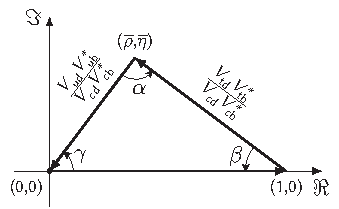
\includegraphics{graphics/intro/tikz/b-d-triangle}
    \caption{}
    \label{fig:unitTriangles_bd}
  \end{subfigure}%
  \begin{subfigure}{0.525\textwidth}
    \raggedleft
    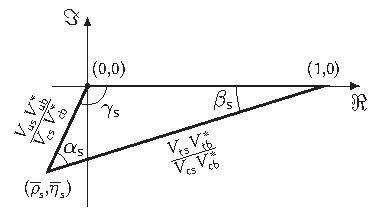
\includegraphics{graphics/intro/tikz/b-s-triangle}
    \caption{}
    \label{fig:unitTriangles_bs}
  \end{subfigure}
  \caption{CKM-unitarity triangles. (a) d--b triangle, corresponding to Equation~\ref{eq:unitConstraints_d}. (b) s--b triangle,
           corresponding to Equation~\ref{eq:unitConstraints_s}.}
  \label{fig:unitTriangles}
\end{figure}

The three terms in each of the orthogonality relations can be used to construct a triangle in the complex plane. The resulting
\emph{unitarity triangles} are schematically shown in Figure~\ref{fig:unitTriangles}. Figure~\ref{fig:unitTriangles_bd} shows the
\emph{d--b triangle}, which corresponds to Equation~\ref{eq:unitConstraints_d}. Its sides are defined by the CKM elements for the couplings
of the up-type quarks and the down/beauty quarks. The angles $\alpha$, $\beta$ and $\gamma$ are defined by
\begin{equation}
  \label{eq:bdAnglesDef}
  \alpha \equiv \arg\left( -\frac{\Vtd\Vtb[*]}{\Vud\Vub[*]} \right)
  \quad
  \beta  \equiv \arg\left( -\frac{\Vcd\Vcb[*]}{\Vtd\Vtb[*]} \right)
  \quad
  \gamma \equiv \arg\left( -\frac{\Vud\Vub[*]}{\Vcd\Vcb[*]} \right)
  \ .
\end{equation}
The coordinates of the triangle apex are defined as $(\rhobar, \etabar)$.

Equation~\ref{eq:unitConstraints_s} gives the \emph{s--b triangle} in Figure~\ref{fig:unitTriangles_bs}. It is defined in a
similar way as the d--b triangle, but its apex has negative real and imaginary coordinates $(\rhosbar, \etasbar)$. The angles $\as$, $\bs$
and $\gs$ are given by
\begin{equation}
  \label{eq:bsAnglesDef}
  \as \equiv \arg\left( -\frac{\Vus\Vub[*]}{\Vts\Vtb[*]} \right)
  \quad
  \bs \equiv \arg\left( -\frac{\Vts\Vtb[*]}{\Vcs\Vcb[*]} \right)
  \quad
  \gs \equiv \arg\left( -\frac{\Vcs\Vcb[*]}{\Vus\Vub[*]} \right)
  \ .
\end{equation}

In Figure~\ref{fig:unitTriangles} the sides of the s--b and d--b triangles were scaled with factors $\Vcd\Vcb[*]$ and $\Vcs\Vcb[*]$,
respectively, to make the first side lie between 0 and 1. Without this scaling, the surface areas of the six possible unitarity triangles
are equal and provide a convention-independent measure of the CP violation that is introduced by the CKM matrix. The areas are given by
half of the \emph{Jarlskog invariant} ($J$) \cite{Jarlskog:1985ht}, which is defined by
\begin{equation}
  \Im( V^{\phantom{*}}_{ij} V^{\phantom{*}}_{kl} V^{*}_{il} V^{*}_{kj} ) \equiv J\; \sum_{m,n} \epsilon_{ikm}\,\epsilon_{jln}
  \ ,
\end{equation}
where $\epsilon$ is the Levi-Civita symbol.

Using the Wolfenstein parameterization and neglecting terms of relative order $\lam^4$ and higher (Equation~\ref{eq:CKMApprox}), the
Jarlskog invariant can be expressed as
\begin{equation}
  J \approx A^2\, \lam^6\, (1-\tfrac{1}{2}\lam^2)\, \eta
  \ .
\end{equation}
Its experimental value is approximately 3\tenpowmult{--5}~\cite{Charles:2004jd,Bona:2005vz}. This value is four orders of magnitude smaller
than the theoretical maximum of $\frac{\text{1}}{\text{6}\sqrt{\text{3}}}$\textapprox0.1 given by unitarity.

In the same relative $\lam^3$ approximation, the only CKM-matrix elements with imaginary parts are $\Vub$, $\Vtd$ and $\Vts$. Using the
approximations of the matrix elements from Equation~\ref{eq:CKMApprox} and the angle definitions from Equations~\ref{eq:bdAnglesDef} and
\ref{eq:bsAnglesDef}, the angles $\gamma$, $\beta$, and $\bs$ are approximated by
\begin{subequations}
  \label{eq:CKMAnglesApprox}
  \begin{alignat}{2}
    \label{eq:CKMGammaApprox}
    \gamma \approx \pi - \gs &\approx \phantom{-}\arg(\Vub[*])
      &&\approx \arctan\left( \frac{\eta}{\rho} \right) \\
    \label{eq:CKMBetaApprox}
    \beta                    &\approx           -\arg(\Vtd)
      &&\approx \arctan\left( \frac{(1-\tfrac{1}{2}\lam^2)\,\eta}{1 - (1-\tfrac{1}{2}\lam^2)\,\rho} \right) \\
    \label{eq:CKMBetasApprox}
    \bs                      &\approx \phantom{-}\arg(-\Vts)
      &&\approx \arctan\left( \frac{\lam^2\,\eta}{1 - \tfrac{1}{2}\lam^2 + \lam^2\rho} \right)
    \ .
  \end{alignat}
\end{subequations}
Expanding the expressions for the angles $\alpha$ and $\alpha_{\text{s}}$ in the same way gives the expected relations between the three
angles in a triangle:
\begin{subequations}
  \begin{alignat}{2}
    \alpha &\approx\, \pi + \arg(\Vtd)  - \arg(\Vub[*]) \,&&\approx\, \pi - \beta - \gamma \\
    \as    &\approx\, \arg(\Vub[*]) - \arg(-\Vts)       \,&&\approx\, \pi - \bs   - \gs
    \ .
  \end{alignat}
\end{subequations}

The experimental values of the CKM angles can be determined by a global fit of the Standard Model to all relevant experimental data. There
are two groups doing such a fit, using different statistical methods and slightly different sets of input data. With the experimental data
that were available in the spring of 2013, the CKMfitter Group finds~\cite{Charles:2004jd}
\begin{equation}
  \label{eq:CKMAnglesCKMf}
  \gamma = (69.7^{+1.3}_{-2.8})^\circ \qquad \beta = (21.8^{+0.8}_{-0.7})^\circ \qquad \bs = (1.05\pm0.04)^\circ
  \ .
\end{equation}

Figures~\ref{fig:unitTriangleMeas_db} and \ref{fig:unitTriangleMeas_sb} show the resulting CKMfitter unitarity triangles, together with the
constrains on the coordinates of the triangle apices. At lowest order in $\lambda$ the apices of the d--b and s--b triangles are given by
$(\rho, \eta)$ and $(-\lam^2\,\rho,\ -\lam^2\,\eta)$, respectively. Constraints from the fit are given by
\begin{equation}
  \label{eq:CKMApicesCKMf}
  \begin{aligned}
    (\rhobar, \etabar)   &= (+0.129^{+0.018}_{-0.009},\ +0.348^{+0.012}_{-0.012}) \\[0.3em]
    (\rhosbar, \etasbar) &= (-0.0068^{+0.0005}_{-0.0010},\ -0.0185^{+0.0006}_{-0.0007})
  \end{aligned}
\end{equation}

\begin{figure}[htbp]
  \centering
  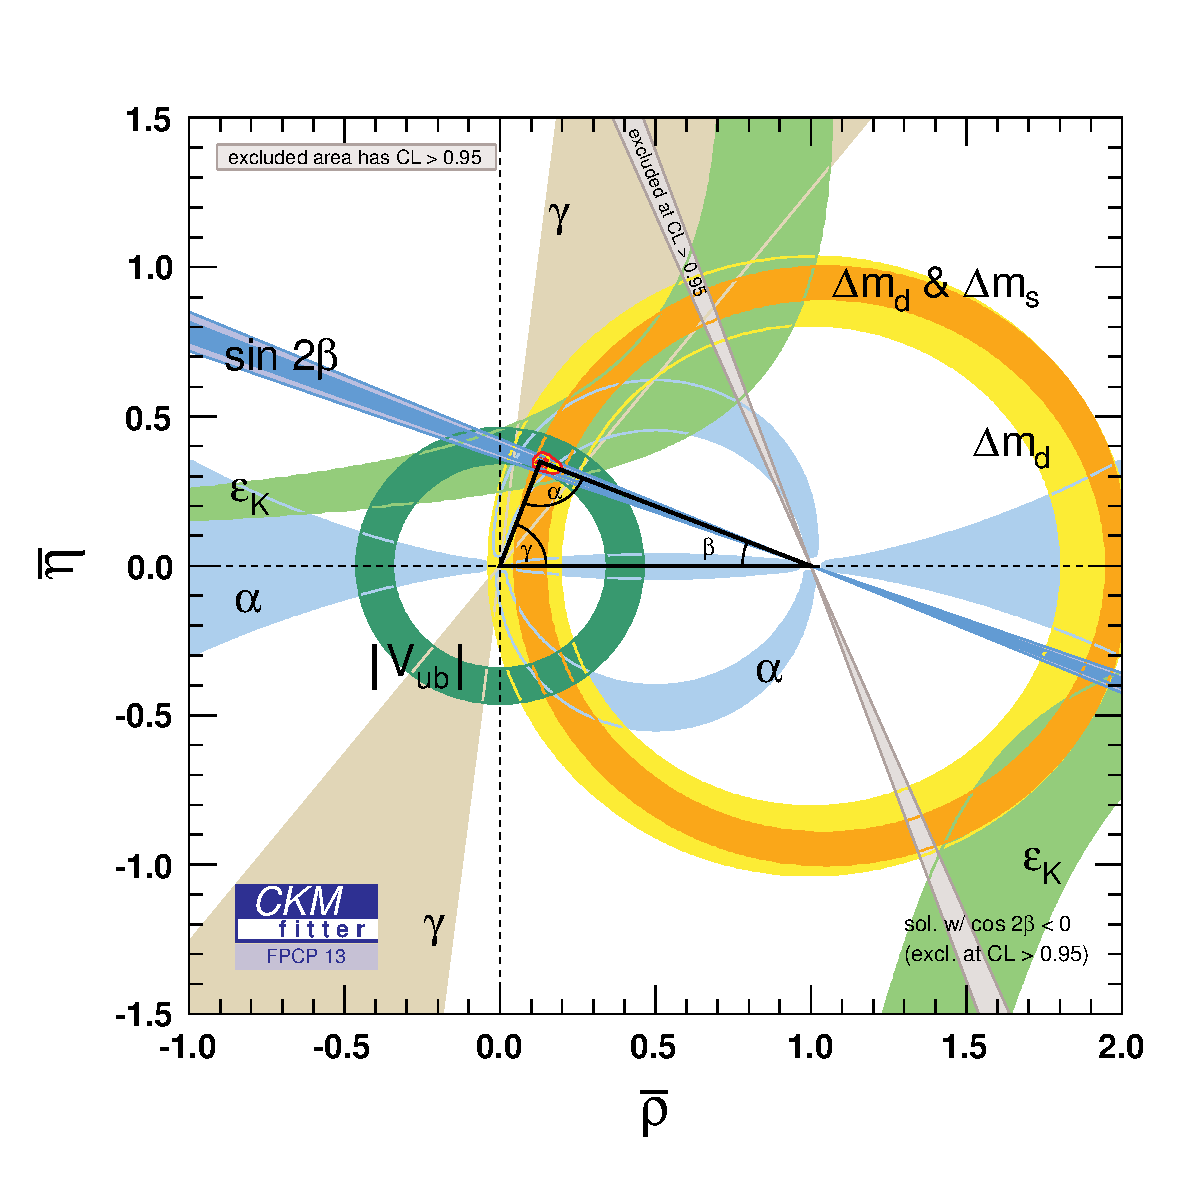
\includegraphics[trim=5mm 2mm 3mm 15mm, clip=true, width=0.8\textwidth]{graphics/intro/rhoeta_large_CMYK}
  \caption{Constraints on the d--b unitarity triangle resulting from the global Standard-Model fit by the CKMfitter Group
           \cite{Charles:2004jd}. The fit estimates the coordinates of the triangle apex in the complex plane, which is given by the
	   parameters $\rhobar\approx\rho$ and $\etabar\approx\eta$.
           Constraints on these parameters from the measurements that are input to the fit are shown as the coloured bands.}
  \label{fig:unitTriangleMeas_db}
\end{figure}

\begin{figure}[htbp]
  \centering
  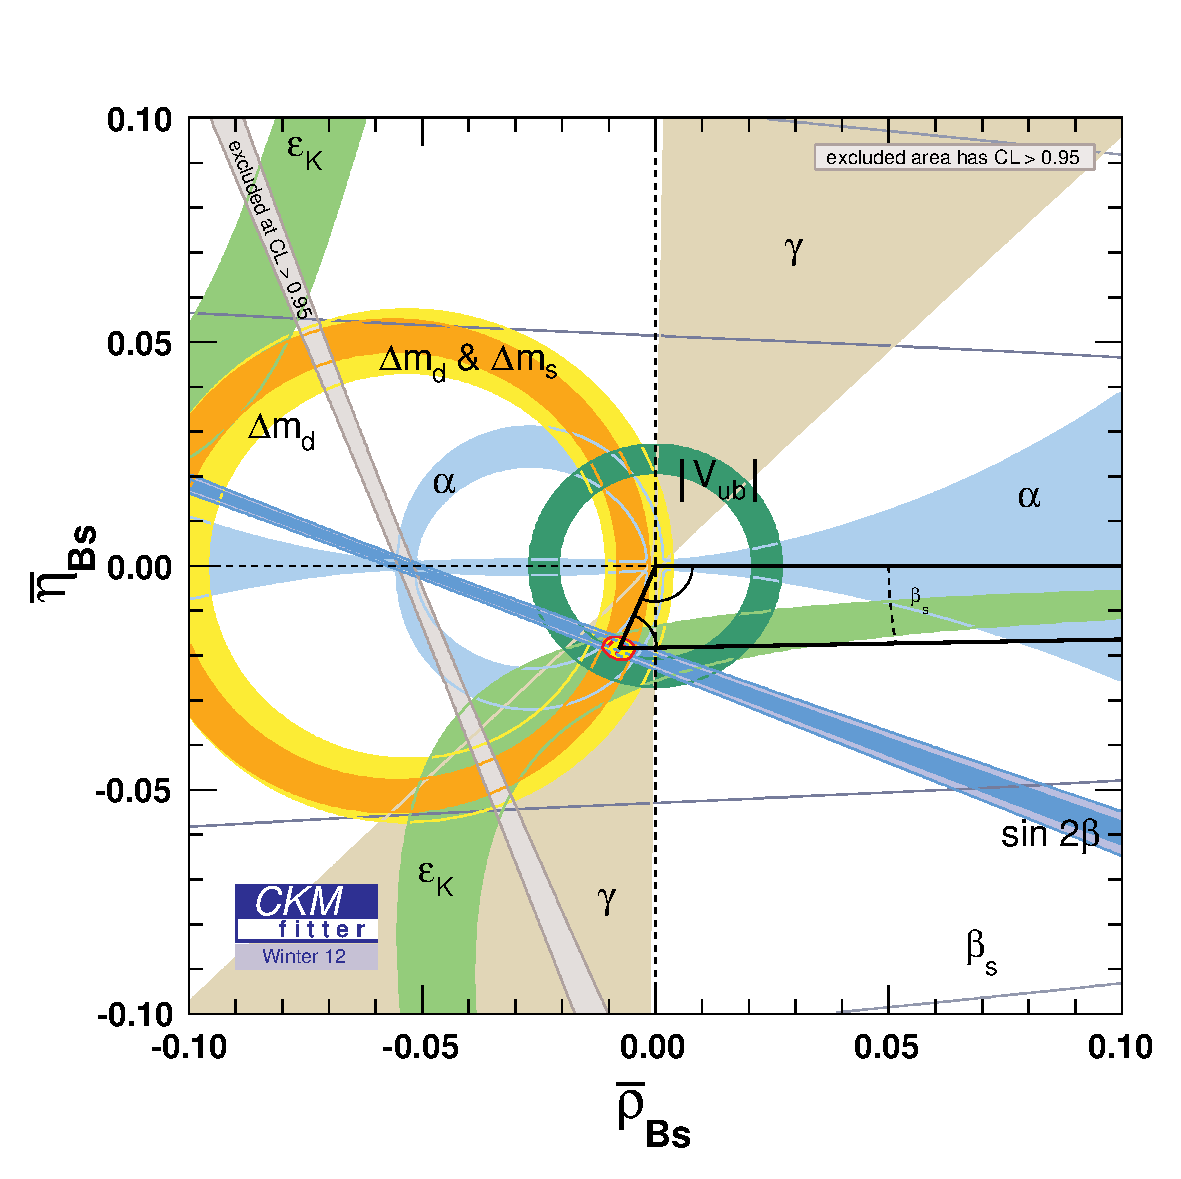
\includegraphics[trim=6mm 2mm 2mm 15mm, clip=true, width=0.8\textwidth]{graphics/intro/rhoBsetaBs_large_global_CMYK}
  \caption{Constraints on the s--b unitarity triangle resulting from the global Standard-Model fit by the CKMfitter Group
           \cite{Charles:2004jd}. The fit estimates the coordinates of the triangle apex in the complex plane, which is given by the
	   parameters $\rhosbar\approx-\lam^2\,\rho$ and $\etasbar\approx-\lam^2\,\eta$.
           Constraints on these parameters from the measurements that are input to the fit are shown as the coloured bands.}
  \label{fig:unitTriangleMeas_sb}
\end{figure}

The UTfit Collaboration finds slightly different values for the angles with the data available by summer 2013~\cite{Bona:2005vz}:
\begin{equation}
  \label{eq:CKMAnglesUTf}
  \gamma = (70.3\pm3.5)^\circ \qquad \beta = (22.0\pm0.9)^\circ \qquad \bs = (1.07\pm0.04)^\circ
  \ .
\end{equation}

Quark-flavour changing interactions and the CKM picture of CP violation provide excellent probes for testing the Standard Model. There are,
for example, measurements that yield one of the CKM angles if only Standard Model processes are considered. If such a measurement gives a
deviation from the value predicted by a global fit or from the value from another measurement, this would be clear evidence for physics
beyond the Standard Model.

As will be discussed in the next section, the CP-violation measurement in the \BstoJpsiphi{} decay yields the phase $\phis$. This phase is
approximately equal to --2$\bs$ in the Standard Model. The value of the angle $\bs$ is very small, since the imaginary part of $\Vts$ is
proportional to a factor $\lam^2$ (see Equations~\ref{eq:CKMApprox} and \ref{eq:CKMBetasApprox}). Even if contributions of unknown new
physics to $\phis$ are small, they could still significantly add to the suppressed Standard Model contribution.

\section{CP Violation in the \texorpdfstring{\BstoJpsiphi{}}{Bs0->Jpsiphi} Decay}
\label{sec:intro_Jpsiphi}

%%%%%%%%%%%%%%%%%%%%%%%%%%%%%%%%%%%%%%%%%%%%%%%%%%%%%%%%%%%%%%%
\subsection{The \texorpdfstring{\BsBsbar{}}{Bs0-Bs0bar} System}
\label{subsec:intro_Jpsiphi_Bs}
%%%%%%%%%%%%%%%%%%%%%%%%%%%%%%%%%%%%%%%%%%%%%%%%%%%%%%%%%%%%%%%

The $\Bs$ meson is a QCD bound state of an anti-b quark and an s quark. Its antiparticle is the $\Bsbar$ meson (b and anti-s). The $\Bs$
and $\Bsbar$ are charge-neutral particles, which makes it possible to convert one into the other. Figure~\ref{fig:mixing} shows the
lowest-order diagrams for this transition.
\begin{figure}[hbt]
  \centering
  \begin{subfigure}{0.5\textwidth}
    \centering
    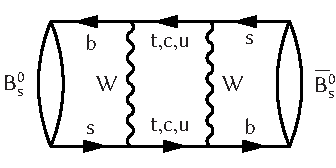
\includegraphics{graphics/intro/box1/box1}
    \caption{}
    \label{fig:mixing_1}
  \end{subfigure}%
  \begin{subfigure}{0.5\textwidth}
    \centering
    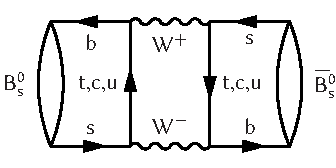
\includegraphics{graphics/intro/box2/box2}
    \caption{}
    \label{fig:mixing_2}
  \end{subfigure}
  \caption{Lowest-order diagrams for \BsBsbar{} mixing (figures from \cite{LHCb-PAPER-2013-002}).}
  \label{fig:mixing}
\end{figure}

Their mixing makes the $\Bs$ and $\Bsbar$ a coupled system of particles. The system comprises two eigenstates with different masses and
mean lifetimes (see Section~\ref{sec:pheno_mix_mix}). A particle that is created as $\Bs$ can at a later point in time be observed as
either a $\Bs$ or a $\Bsbar$. As a result, the distribution of the time at which the \BsBsbar{} system decays is not a simple exponential,
as it would be in the absence of mixing. Because the expression for the probability to observe the system as a $\Bs$ or a $\Bsbar$ as a
function of time contains sinusoidal terms, mixing is often referred to as ``\BsBsbar{} oscillations''.

The \emph{decay time} is defined as the elapsed time between the production and the decay of the \BsBsbar{} system in its rest frame. In
Section~\ref{sec:pheno_mix} the exact shape of the decay-time dependence will be discussed. The applied formalism is common to the $\Dmes$,
$\Bd$ and $\Bs$ mesons and, to some extend, also the $\kaon$ meson, which all mix with their respective antiparticles.

The parameters used to describe the \BsBsbar{} system are the mean decay width, $\Gs$, the difference between the decay widths of the
eigenstates, $\DGs$, and the difference between the masses of the eigenstates, $\Dms$. By definition, the mean lifetime of the system is
given by $\taus$\textequiv$\frac{\text{1}}{\Gs}$. The mass difference will turn out to be the frequency of the oscillations of the
\BsBsbar{} probability in time.

In the Standard Model, CP violation enters the mixing process through the CKM-matrix elements at W-boson vertices. The amplitudes in
Figure~\ref{fig:mixing} depend on the mass of the internal up-type quark, which makes the \BsBsbar{} mixing process dominated by diagrams
with virtual top quarks. As a result, CP violation is small, since it requires multiple contributions with different weak phases. In terms
of Equation~\ref{eq:interference}, this corresponds to a small value of $R$, which suppresses the CP asymmetry.

The additional contributions that do give rise to small \emph{CP violation in mixing} are transitions via real intermediate states into
which both $\Bs$ and $\Bsbar$ can decay, which will be discussed in more detail in Section~\ref{sec:pheno_mix}. The asymmetry between the
$\Bs\to\Bsbar$ and $\Bsbar\to\Bs$ rates is measured to be approximately one per cent~\cite{Amhis:2012bh}. Given the current experimental
uncertainties, this is compatible with no CP violation.

Depending on the final state, there may also be different amplitudes contributing to the decay of the $\Bs$ meson. Also then
interference can lead to different decay rates, in this case for the $\Bstof$ and $\Bsbartofbar$ processes. This form is termed \emph{CP
violation in decay}.

The first significant observation of CP violation in the $\Bs$ system was recently obtained by LHCb~\cite{LHCb-PAPER-2013-018}. This was a
measurement of CP violation in decay for $\Bsbar\to\Kp\pimes[-]$ and $\Bs\to\Km\pimes[+]$, where an asymmetry in the decay rates of about
30\% was found.

\newcommand{\ffig}{\fp}
\newcommand{\phimixfig}{\phi_\text{mix}}
\newcommand{\phifig}{\phi_\text{dec}}
\newcommand{\phibarfig}{\kern 0.15em \overline{\kern -0.15em \phi_\text{dec} \kern -0.60em} \kern 0.60em}
\begin{figure}[tb]
  \centering
  \resizebox{0.4\textwidth}{!}{\input{graphics/intro/decay.pdftex_t}}
  \caption{Interference between the $\Bstof[\fp]$ and $\Bs\to\Bsbartof[\fp]$ processes. The phases $\phimixfig$, $\phifig$, and
           $\phibarfig$ are the relevant weak phases contributing to the two decay paths from the mixing, $\Bs$ decay and $\Bsbar$ decay,
           respectively. This is assuming no CP violation in mixing or CP violation in decay.}
  \label{fig:interference}
\end{figure}

An interesting situation occurs if both $\Bs$ and $\Bsbar$ can decay into the same final state $\fp$. In that case the processes
$\Bstof[\fp]$ and $\Bs\to\Bsbartof[\fp]$ interfere, which is depicted schematically in Figure~\ref{fig:interference}. Even without CP
violation in mixing or CP violation in decay, the interference of these two decay paths may cause a difference between the rates of
$\Bs(\to\Bsbar)\to\fp$ and $\Bsbar(\to\Bs)\to\overline{\fp}$. This difference is called \emph{CP violation in the interference of decays
with and decays without mixing}.

Interference between the decays with and without mixing leads to a CP asymmetry that depends on the decay time. A sinusoidal term is
introduced in the differential decay rate as a function of decay time with an amplitude that depends on the amount of CP violation. This
oscillation originates from the time dependence of the transition amplitudes in \BsBsbar{} mixing and consequently has a frequency equal to
the mass difference $\Dms$. In an experiment it is important to resolve the resulting oscillation in the decay-time distribution, which
enables the measurement of its amplitude and hence the amount of CP violation.

A special case of this form of CP violation is the one where $\fp$ is a CP eigenstate. In this case $\fp$ and $\overline{\fp}$ are
identical and CP violation results in a difference between the decay rates of $\Bs(\to\Bsbar)\to\fp$ and $\Bsbar(\to\Bs)\to\fp$.

An example of such a decay is the so-called ``golden mode'' \BdtoJpsiKS. The combination of CKM-matrix elements from $\Bd$--$\Bdbar$ mixing
and the \BdtoJpsiKS{} decay makes the amplitude of the oscillations in decay time depend on the CKM angle $\beta$. The measurement of
$\beta$ with this decay mode by the BaBar and Belle experiments~\cite{Aubert:2001nu,*Abe:2001xe} was the first observation of CP violation
in $\Bd$ decays. The result of combining all currently available measurements of the angle $\beta$~\cite{Amhis:2012bh} is consistent with
the value obtained from the global Standard Model fits~\cite{Charles:2004jd,Bona:2005vz}.


%%%%%%%%%%%%%%%%%%%%%%%%%%%%%%%%%%%%%%%%%%%%%%%%%%%%%%%%%%%%%%%%
\subsection{\texorpdfstring{\BstoJpsiphi{}}{Bs0->Jpsiphi} Decay}
\label{subsec:intro_Jpsiphi_decay}
%%%%%%%%%%%%%%%%%%%%%%%%%%%%%%%%%%%%%%%%%%%%%%%%%%%%%%%%%%%%%%%%

The \BstoJpsiphi{} decay%
\footnote{Charge-conjugate particles, CP-conjugate decays and neutral-meson mixing are implied, unless stated otherwise.}
of the $\Bs$ system is equivalent to the \BdtoJpsiKS{} decay of the $\Bd$ system. Its decay-time distribution depends on the angle $\bs$
instead of $\beta$, as will be shown below.

However, in comparison to \BdtoJpsiKS, a complication arises from the fact that both the $\Jpsi$ and the $\phimesalt$ are spin-one mesons,
whereas the $\KS$ is a spin-zero meson. This leads to three possible orbital angular momentum configurations of the $\Jpsiphi$ system,
compared to one configuration for the $\Jpsi\,\KS$ system. As a result, the \BstoJpsiphi{} decay comprises three different CP eigenstates
instead of one. The contributions of these states must be statistically separated by an analysis of the $\Jpsi$ and $\phimesalt$ spin
polarizations for an optimal measurement~\cite{Dighe:1995pd,Dighe:1998vk}, as will be explained in Section~\ref{sec:pheno_decay}.

\begin{figure}[hbt]
  \centering
  \begin{subfigure}{0.5\textwidth}
    \centering
    \begin{tikzpicture}
      \node[anchor=south]{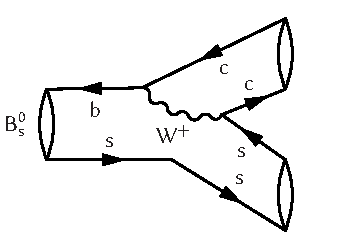
\includegraphics[clip=true, trim=0mm 3mm 0mm 3mm]{graphics/intro/tree/tree}};
      \node[anchor=west] at (1.95, 3.17) {\sffamily$\Jpsi$};
      \node[anchor=west] at (1.95, 0.75) {\sffamily$\phimesalt$};
    \end{tikzpicture}
    \caption{}
    \label{fig:decay_tree}
  \end{subfigure}%
  \begin{subfigure}{0.5\textwidth}
    \centering
    \begin{tikzpicture}
      \node[anchor=south]{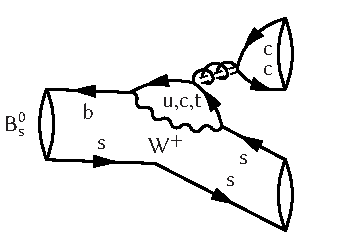
\includegraphics[clip=true, trim=0mm 3mm 0mm 3mm]{graphics/intro/penguin/penguin}};
      \node[anchor=west] at (1.95, 3.17) {\sffamily$\Jpsi$};
      \node[anchor=west] at (1.95, 0.75) {\sffamily$\phimesalt$};
    \end{tikzpicture}
    \caption{}
    \label{fig:decay_penguin}
  \end{subfigure}
  \caption{\BstoJpsiphi{} decay (figures from \cite{LHCb-PAPER-2013-002}): (a) tree-level diagram; (b) penguin diagram.
           The curled/dashed line in (b) represents a colour-neutral state, which can be a Z$^0$, a photon, or colour-singlet gluons.}
  \label{fig:decay}
\end{figure}
At quark level, the \BstoJpsiphi{} decay is a \emph{$\btoccs$ transition}. The b quark decays into an s quark and a c$\qbar[c]$ pair, where
the s quark forms a $\phimesalt$ meson with the spectator $\qbar[s]$ quark and the c$\qbar[c]$ pair forms a $\Jpsi$ meson.
Figure~\ref{fig:decay_tree} shows the dominant Standard Model contribution. This is a tree-level diagram, which is proportional to the
CKM-matrix elements $\Vcs$ and $\Vcb[*]$.

Since the CP-violation phenomenology is governed by \BsBsbar{} mixing and the $\btoccs$ transition, decays in which the c$\qbar[c]$ and
s$\qbar[s]$ pairs form different mesons may be used in addition to \BstoJpsiphi. An example is the \BstoJpsipipi{}
decay~\cite{Stone:2008ak}, which is also used by LHCb to measure $\phis$.

The dominant contributions to the \BsBsbar{} mixing with internal top quarks (Figure~\ref{fig:mixing}) are proportional to
$(\Vts\Vtb[*])^2$. In combination with the tree-level decay, these give a weak phase difference between decays with and decays without
mixing of
\begin{equation}
  \label{eq:betasCKM}
  \begin{split}
    &\arg\left[(\Vts\Vtb[*])^2\right] + \arg\left(\Vcs[*]\Vcb\right) - \arg\left(\Vcs\Vcb[*]\right) \\
    &\qquad\qquad= 2\,\arg\left(-\frac{\Vts\Vtb[*]}{\Vcs\Vcb[*]}\right) = 2\bs
    \ ,
  \end{split}
\end{equation}
where the first contribution comes from the $\Bs\to\Bsbar$ transition, the second contribution from the subsequent $\Bsbar$ decay, and the
third contribution from the $\Bs$ decay path without mixing.

Additional contributions to the mixing and decay processes can affect this prediction of the weak phase. The quantity that is observed in
this measurement is the phase $\phis$, which is equal to --2$\bs$ with the above assumptions.%
\footnote{There are various, often contradicting notations of the phase difference in use. In this work $\bs$ is the CKM-triangle angle
(Equation~\ref{eq:bsAnglesDef}) and $\phis$ the model-independent observable (see Sections~\ref{sec:pheno_decay} and
\ref{subsec:pheno_time_commonCPV}). If only dominant Standard Model contributions to both mixing and decay are considered, $\phis$ is equal
to --2$\bs$.}

In the Standard Model, corrections come from the mixing diagrams with real states and from higher order contributions to the decay.  While
the former lead to small Standard Model CP violation in mixing, these amplitudes are not expected to contribute significantly to the value
of $\phis$ (see Section~\ref{sec:pheno_mix_obs}). An example of an additional contribution to the decay is the \emph{penguin diagram} in
Figure~\ref{fig:decay_penguin}. Although hard to estimate, small contributions from penguin diagrams to the decay are
expected~\cite{Faller:2008gt,*Bhattacharya:2012ph}.

Apart from CP violation in the interference between decays with and decays without mixing, the \BstoJpsiphi{} process is affected by CP
violation in mixing and by CP violation in decay. As discussed above, CP violation in mixing is small and its effects are not expected to
be measurable in the \BstoJpsiphi{} measurement. CP violation in decay arises from interference between different decay amplitudes. Since
the decay is dominated by the tree-level amplitude, also CP violation in decay is expected to be small in the \BstoJpsiphi{} process.

Beyond the Standard Model, CP violation can arise from new contributions to the \BsBsbar{} mixing
process~\cite{Nir:1990hj,*Silverman:1998uj,*Ball:1999yi,*Dunietz:2000cr,Buras:2009if} as well as the $\Bs$
decay~\cite{Chiang:2009ev,*Datta:2009fk}. In general it is expected that potential corrections to the Standard Model are largest in
processes with virtual particles in loops at lowest order. Loop processes are smaller than tree-level processes, which makes Standard Model
contributions compete with potential new contributions at the same level. New particles must be heavy and cannot be created in decays of
Standard Model particles. In loop processes, however, they can enter as virtual particles and replace, for example, the internal top quarks
in the \BsBsbar{} mixing diagrams. For these reasons, the focus of the measurement will be on mixing-induced CP violation rather than CP
violation that arises from the \BstoJpsiphi{} decay, which is dominated by the tree-level amplitude in Figure~\ref{fig:decay_tree}.

If the effect of new contributions on the value of $\phis$ is large compared to the Standard Model prediction, the corresponding deviation
can be revealed by the measurement of a large non-zero value of $\phis$. In this case an exact estimate of the Standard Model value is not
required and subleading penguin contributions can be neglected. Such a large deviation could be detected by a low-statistics measurement,
which would not have the precision to distinguish between the cases of no CP violation, the Standard Model, and a small deviation from the
Standard Model.

Measurements of $\phis$ with the \BstoJpsiphi{} decay prior to this thesis have been performed by the D0~\cite{Abazov:2011ry},
CDF~\cite{Aaltonen:2012ie}, \atlas~\cite{Aad:2012kba,*ATLAS:2013nla}, and LHCb~\cite{LHCb-PAPER-2013-002} experiments. LHCb also measured
$\phis$ in the \BstoJpsipipi{} decay channel~\cite{LHCb-PAPER-2014-019}. All measurements and their combination~\cite{Amhis:2012bh} are
compatible with no CP violation and also with the value of $\bs$ from the Standard Model fit. The LHCb measurement in the \BstoJpsiphi{}
channel yielded
\begin{equation}
  \label{eq:phis1fb}
  \phis\text{\texteq+0.07\textpm0.09$\,$(stat.)\textpm0.01$\,$(syst.)~~rad\ ,}
\end{equation}
where the first uncertainty is statistical and the second systematic. This value is to be compared with the Standard Model estimate
--2$\bs$\texteq--0.0368$^\text{+0.0013}_\text{--0.0014}$\unitsp{}rad (see Equation~\ref{eq:CKMAnglesCKMf} and
reference~\cite{Charles:2004jd}).

A measurement of the decay-time distribution in \BstoJpsiphi{} is not only sensitive to the phase $\phis$, but also to the lifetime
parameters of the \BsBsbar{} system. The previously mentioned CP violation measurements yielded estimates of $\Gs$ and $\DGs$ as well.
These parameters were also estimated by CMS in a measurement that assumed no CP violation~\cite{CMS:2012pca}.

In the Standard Model the parameter $\Gs$ is expected to be equal to the $\Bd$ decay width, $\Gd$, up to relative corrections of the order
of \tenpow{--3}~\cite{Lenz:2006hd,*Lenz:2011ti}. $\Gd$ is measured to be 0.6583\textpm0.0030\unitsp\invps~\cite{Amhis:2012bh}. A prediction
of the decay-width difference $\DGs$ yields 0.087\textpm0.021\unitsp\invps~\cite{Lenz:2006hd,*Lenz:2011ti}. The measurements of $\Gs$ and
$\DGs$ and their combination~\cite{Amhis:2012bh} are compatible with these predictions. The estimates from the LHCb measurement are given
by
\begin{subequations}
  \label{eq:width1fb}
  \begin{align}
    \label{eq:avWidth1fb}
    \Gs&\text{\texteq0.663\textpm0.005$\,$(stat.)\textpm0.006$\,$(syst.)~~\invps} \\
    \label{eq:diffWidth1fb}
    \DGs&\text{\texteq0.100\textpm0.016$\,$(stat.)\textpm0.003$\,$(syst.)~~\invps\ .}
  \end{align}
\end{subequations}

\begin{figure}[tb]
  \centering
  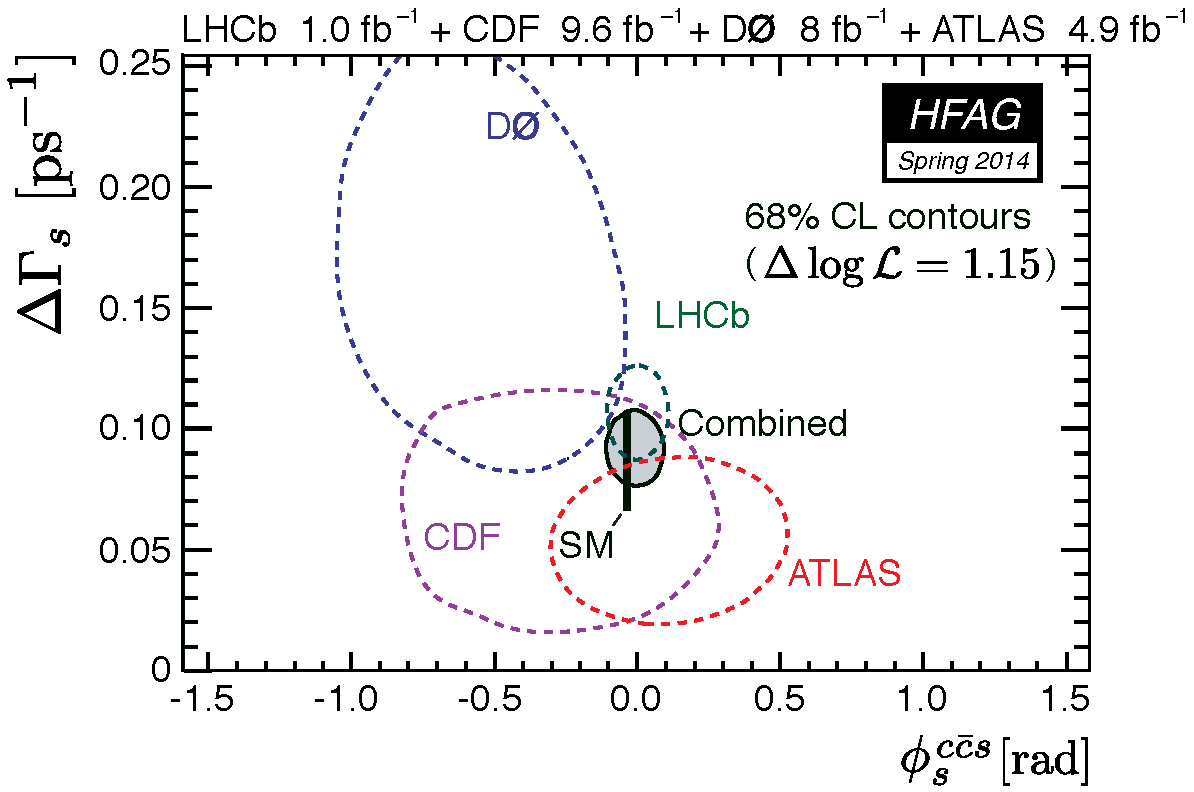
\includegraphics[width=0.8\textwidth]{graphics/intro/hfag_spr2014_DGsphis_comb-crop-cmyk}
  \caption{Combination of $\phis$ (here represented as $\phisccs$) and $\DGs$ measurements by HFAG~\cite{Amhis:2012bh}.
           The estimates at 68\% confidence level (CL) by the different experiments are shown by the dashed contours.
           Note that the LHCb contour is a combination of measurements in the \BstoJpsiphi{} and \BstoJpsipipi{} decays.
           The combined 68\% confidence region is shown by the shaded area and the Standard Model prediction by the vertical bar.}
  \label{fig:phisDGs}
\end{figure}
A graphical representation of the status of $\phis$ and $\DGs$ measurements in the spring of 2014 by the Heavy Flavour Averaging Group
(HFAG) is shown in Figure~\ref{fig:phisDGs}. The LHCb contribution is a combination of the \BstoJpsiphi{} and \BstoJpsipipi{} results with
data from 2011, which form roughly one third of the currently available dataset. The 68\% confidence-level (CL) contour of the combined
result is consistent with the region that represents the Standard Model prediction.

As it is clear from Figure~\ref{fig:phisDGs} that possible effects from non-Standard Model physics on $\phis$ and $\DGs$ cannot be large,
more precise measurements are required to probe them. With the currently available LHCb data, combination of the $\phis$ estimates from the
two decay channels is expected to reach a precision of approximately 0.04~rad, which is roughly equal to the value of the Standard Model
prediction. An improvement of this precision by an order of magnitude is expected with future LHCb data.

For a measurement with this precision, effects have to be taken into account that have not been considered for previous measurements. A
precise estimate of Standard Model CP violation is required, which also includes higher order penguin contributions to the $\btoccs$
transition. A complication arises from the fact that these additional contributions affect the value of $\phis$ differently for the
\BstoJpsiphi{} and \BstoJpsipipi{} decays and for the different intermediate states that contribute to the
decays~\cite{Faller:2008gt,*Bhattacharya:2012ph}. Moreover, physics beyond the Standard Model may also affect all intermediate states
differently~\cite{Chiang:2009ev,*Datta:2009fk}. These effects need to be considered not only in theoretical predictions, but also in
measurements.

In the \BstoJpsiphi{} measurement that is presented in this thesis the dependence of CP violation on the intermediate state is taken into
account for the first time. The value of $\phis$ is estimated separately for each of the CP eigenstates in the decay, which is possible
if the contributions of the states are statistically separated. The decay model for this measurement is presented in
Chapter~\ref{chap:pheno}.


%%%%%%%%%%%%%%%%%%%%%%%%%%%%%%%%%%%%%%%%%%%%%%%%%%%%%%%%%%%%%%%%%%%
\subsection{The \texorpdfstring{$\mumuKK$}{mu+mu-K+K-} Final State}
\label{subsec:intro_Jpsiphi_final}
%%%%%%%%%%%%%%%%%%%%%%%%%%%%%%%%%%%%%%%%%%%%%%%%%%%%%%%%%%%%%%%%%%%

The $\Jpsiphi$ system is unstable and only its decay products can be detected. There are many possibilities for both the $\Jpsi$ and
$\phimesalt$ mesons to decay~\cite{PDG}. The only final state that will be considered here is $\mumu\,\KK$, where the muon pair
originates from the $\Jpsi$ decay and the kaon pair from the $\phimesalt$ decay. All four particles can be detected efficiently and with
low background by the LHCb detector, as will be described in Section~\ref{sec:intro_LHCb}. This makes \BstoJpsimumuphiKK{} the optimal
channel to measure CP violation in $\Bs$ decays with a $\btoccs$ transition.

Since the $\mumuKK$ final state can also be reached through resonances other than the $\Jpsi$ and the $\phimesalt$, interference with other
processes needs to be considered. To optimize for the detection of the $\Jpsi$ and $\phimesalt$ resonances, a region in kinematic phase
space is selected where this intermediate state dominates.

The measured invariant mass of the muon pair is required to be between 3.03 and 3.15~\GeV{} (see also Section~\ref{sec:ana_bkgSub}).
%\footnote{The unit of energy used in particle physics is the \emph{electronvolt} (eV), which is approximately equal to
%1.6\tenpowmult{--19}~J. Derived units for momentum and mass are \eVc{} and \eV, respectively, where $c$ is the speed of light.}
This restriction is assumed to select only those \BstomumuKK{} decays with muons coming from a $\Jpsi$, which has a mass of approximately
3.10~\GeV{}~\cite{PDG}.

Also the invariant-mass range of the $\KK$ pair is restricted, but there the situation is more complicated. An analysis of the resonant
components in the $\KK$ system~\cite{LHCb-PAPER-2012-040} has shown that there is a mass region where the $\phimes$ dominates, but other
contributions cannot be neglected.

\begin{figure}[tbp]
  \centering
  %\begin{tikzpicture}[line width=0.08em]
  %  \node [anchor=south] {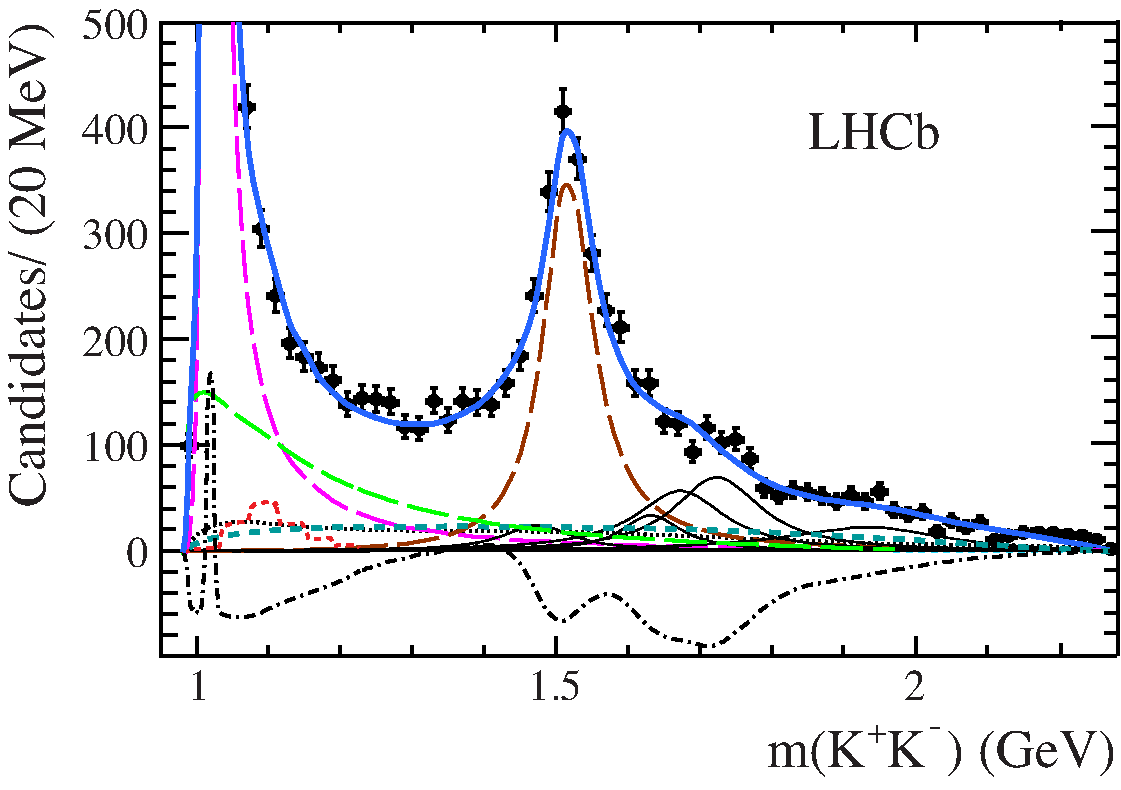
\includegraphics[width=0.7\textwidth]{graphics/intro/KKComponents}};
  %  \draw[red] (-0.2047\textwidth,0.04\textwidth) -- (-0.2047\textwidth,0.52\textwidth);
  %\end{tikzpicture}

  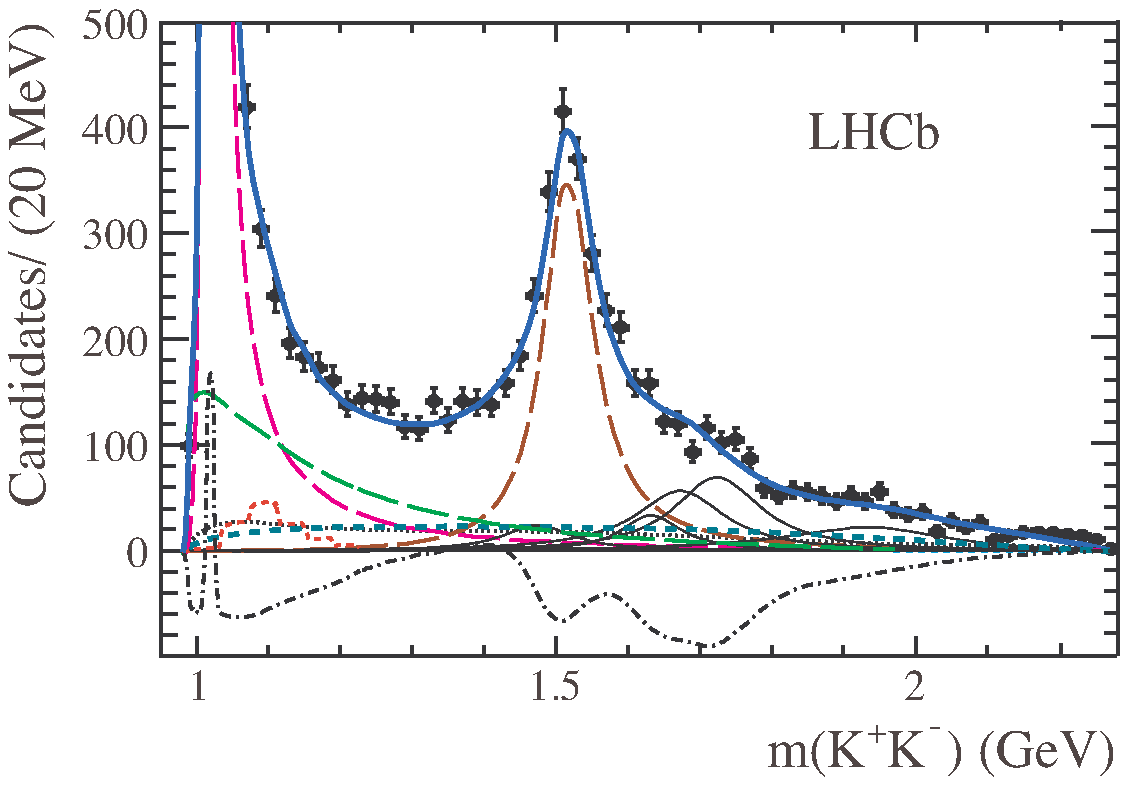
\includegraphics[width=0.9\textwidth]{graphics/intro/KKComponents-cmyk}
  \caption{$\KK$-mass spectrum in \BstoJpsiKK{} decays~\cite{LHCb-PAPER-2012-040}. The black points represent a histogram of decay
           candidates.
           %, where the size of the error bar shows the fluctuation expected from a Poisson distribution of the number of entries
           %in each mass bin.
           A model of the mass distribution is shown as the blue curve. The largest contributions to the distribution
           come from the $\phimes$, $\ftwop$, and $\fzero$ resonances, which are shown as the magenta,
           brown, and green, long-dashed lines, respectively. Notice that a large part of the $\phimes$ peak is not visible,
           because of the truncated vertical scale.
           Other resonances (heavier $\phimesalt$, $\fzeroalt$, and $\ftwoalt$ states) are shown as the thin, black curves
           and a non-resonant contribution as the dashed, cyan curve.
           The contribution from interferences between the resonances is represented by the dotted-dashed, black line.
           The small dotted, black and dashed, red contributions are backgrounds of four
           particles that do not originate from a \BstoJpsiKK{} decay.}
           %The region to the left of the vertical, red line is dominated by the $\phimes$.}
  \label{fig:KKComponents}
\end{figure}

The $\KK$-mass spectrum in \BstoJpsiKK{} decays is shown in Figure~\ref{fig:KKComponents}. The contribution of the $\phimes$ is represented
by the dashed, magenta curve. Notice that part this peak is not visible, because of the truncated vertical scale.

For the \BstoJpsiphi{} CP-violation measurement, only $\KK$ pairs with a mass between 0.99 and 1.05~\GeV{} are selected. In this region the
$\phimes$ clearly dominates, but there are also contributions from the $\fzero$ and from $\KK$ pairs that do not originate from the decay
of a resonance.

For both the $\fzero$ and non-resonant contributions the $\KK$ system is in a state of zero orbital angular momentum and hence these
contributions are commonly referred to as the \emph{$\KK$ S-wave}. Because the $\phimes$ is a spin-one particle, the orbital angular
momentum of the $\KK$ system has an orbital angular momentum equal to one for the $\Jpsiphi$ intermediate state. Therefore, the
\BstoJpsiphi{} contribution is sometimes termed \emph{$\KK$ P-wave}. Since the $\Jpsiphi$ and $\KK$ S-wave processes are observed
simultaneously in the measurement, the analysed decay is referred to as \BstoJpsiKK.

In addition to separating the three components of the \BstoJpsiphi{} process, these components are also separated from the $\KK$ S-wave
contribution. The latter could be accomplished on a statistical basis with an analysis of the $\KK$-mass distribution. However, this
distribution does not discriminate between the CP eigenstates of the \BstoJpsiphi{} decay, so a different approach is chosen.

The spatial distributions of the final-state particles are different for the \BstoJpsiphi{} and $\KK$ S-wave contributions, which enables a
statistical separation of the two components. An analysis of the spatial distributions also separates $\Jpsiphi$ spin-polarization states
and hence the three CP eigenstates of this system.

The directions of the final-state particles are specified with respect to the momentum directions of the $\mumu$ and $\KK$ systems in the
centre-of-mass system of the $\Bs$ meson. This is done with three \emph{decay angles}, which can be computed given the four-momenta of the
final-state particles. These angles are included in the model of the decay, in addition to the decay time. The formalism for the angular
dependence of the decay is described in detail in Section~\ref{sec:pheno_angles} and Appendix~\ref{chap:angularDecay}.

\section{The \texorpdfstring{\BstoJpsiKK}{Bs0->J/psi K+K-} Decay in LHCb}
\label{sec:intro_LHCb}

%%%%%%%%%%%%%%%%%%%%%%%%%%%%%%%%%%%%%%%%%%%%%%%%%%%%%%%%%%%%%%%%%%%%%%%%%%%%%%%%%%%%%%
\subsection{\texorpdfstring{$\Bs$}{Bs0}-Meson Production at the Large Hadron Collider}
\label{subsec:intro_LHCb_LHC}
%%%%%%%%%%%%%%%%%%%%%%%%%%%%%%%%%%%%%%%%%%%%%%%%%%%%%%%%%%%%%%%%%%%%%%%%%%%%%%%%%%%%%%

The $\Bs$ mesons that are used for the \BstoJpsiKK{} measurement are produced in the proton--proton collisions of the Large Hadron Collider
(LHC) \cite{Evans:2008zzb}. The LHC accelerates protons to high energies and makes them collide head-on at designated points. For the
measurement presented here, data from the LHC data-taking runs 2011 and 2012 were used. In 2011 colliding protons had an energy of
3.5\unitsp{}TeV, while the energy was increased to 4\unitsp{}TeV for 2012. This gave a centre-of-mass energy in proton--proton collisions
of 7 and 8\unitsp{}TeV, respectively.

Protons are brought to an energy of 0.45\unitsp{}TeV by a series of pre-accelerators before they are injected into the LHC. There they are
stored in two opposite, circular beams and accelerated to the collision energy. Each beam contained 1380 bunches of \tenpow{11} protons in
most of the 2011 and 2012 runs.

When the collision energy is reached, the beams are tuned to make bunches collide at four distinct \emph{interaction points}, where the
detectors of the LHC experiments are located. The moment at which two bunches meet is called a \emph{bunch crossing}. If proton--proton
collisions in a bunch crossing produce particles that are of interest for an experiment, this is called an \emph{event}. After typically
ten hours of collisions the number of remaining protons in the beams becomes too small to maintain a sufficiently high collision rate and
the beams are dumped to restart the cycle of acceleration and collisions.

The mean number of collisions per bunch crossing that produce detectable particles at the LHCb interaction point varied between one and two
in 2011 and 2012. This number is determined by the probability that two protons interact when they pass each other and by the probability
that the protons get close enough to enable such an interaction. These probabilities are represented by two effective quantities: the
proton--proton \emph{cross section} and the beam \emph{luminosity}.

The luminosity is an effective density of protons that meet each other per unit of time across a surface perpendicular to the beams at the
interaction point. This quantity is fully determined by the beam parameters, in particular by the number of protons per bunch and the
number of bunch crossings per unit time. To get a quantity that represents the total number of protons that passed each other per unit
surface, the luminosity is integrated over time. The integrated luminosity is 1\unitsp\invfb{} for 2011 and 2\unitsp\invfb{} for 2012.
%\footnote{Surface areas in this context are measured in units of \emph{barn} (b):
%1\unitsp{}b\textequiv\tenpow{--28}\unitsp{}m\textsuperscript{2}.}

To obtain the number of interactions per unit time, the luminosity is multiplied by the surface area of the effective proton cross section.
This surface area represents the strength of the interaction between the colliding particles, which typically depends on the centre-of-mass
energy of the collision.

The total proton--proton cross section is a sum of the cross sections for all possible interactions, which can be elastic or inelastic.
While elastic interactions do not break up the colliding protons, inelastic interactions do and create new particles. The latter type is
relevant for the production of $\Bs$ and $\Bsbar$ mesons.

The sum of the cross sections for $\Bs$ and $\Bsbar$ production in LHCb is measured to be approximately 1\tenpowmult{10}\unitsp{}fb at an
energy of 7\unitsp{}TeV \cite{LHCB-PAPER-2013-004}. Assuming the cross section at 8\unitsp{}TeV is approximately the same, this gives a
total of 3\tenpowmult{10} produced $\Bs$ and $\Bsbar$ mesons in 2011 and 2012. A fraction of 3\tenpowmult{--5} decays into $\JpsimumuphiKK$
\cite{PDG}, which yields an expected number of 9\tenpowmult{5} decays. Including particle-detection inefficiencies and selection of
usable decays, about 9\tenpowmult{4} decays are left for analysis (see Section\unitsp{}\ref{sec:exp_selBkg}).

To produce $\Bs$ and $\Bsbar$ mesons, (anti)beauty and (anti)strange quarks must be created. Beauty quarks are predominantly produced as
$\bbbar$ pairs. Beauty hadrons are formed by combining the b and $\qbar[b]$ quarks with lighter quarks that are produced at a later stage.
If this lighter quark is an s ($\qbar[s]$) quark, the result is a $\Bs$ ($\Bsbar$) meson.

In the inelastic collisions that are relevant for $\bbbar$ production, the constituents of the colliding protons interact. These
constituents can be (anti)quarks or gluons, which are collectively called \emph{partons}. A proton consists of three valence quarks: two up
quarks and one down quark. In addition it contains virtual partons, created by low-energy, non-perturbative QCD interactions. The
centre-of-mass energy of the collision is large enough to make the lifetime of these virtual states larger than the time needed to also
interact with partons from the other proton.

The colliding protons break up in the parton interaction, leaving coloured remnants. Quarks and gluons created in the interaction and
these proton remnants recombine into colourless hadrons. This process is called \emph{hadronization}. Tens of hadrons can be created in a
single proton--proton collision at the LHC.

The energy carried by a parton is a fraction of the proton energy. For $\bbbar$ production the energy fractions of the interacting partons
must be minimally the ratio of the energy to produce beauty-hadron masses and the collision energy, which is of the order of \tenpow{--3}.
However, in most collisions the fractions are different for the two interacting partons. This gives the produced particles additional
energy and leads to large boosts along the beam direction.

Conceptually the parton interaction can be separated into two parts. First there are high-energy interactions, which are described by
perturbative QCD. The proton energy is converted into particle masses, which may be much larger than the proton mass. Beauty quarks are
created at this stage.

Interactions that follow are less energetic and create only lighter quarks in quark--antiquark pairs. This non-perturbative process is
called \emph{fragmentation}. A $\Bs$ meson is formed with the strange quark from a created s$\qbar[s]$ pair. The remaining antistrange
quark forms a hadron with other quarks in the fragmentation process.

The $\Bs$ production mechanism can be exploited to determine whether the produced meson was a $\Bs$ or a $\Bsbar$. This procedure is called
\emph{flavour tagging}. The flavour information cannot be inferred directly from the decay into $\mumuKK$, since both $\Bs$ and $\Bsbar$
decay into this charge-neutral final state. For the CP-violation measurement in \BstoJpsiKK, however, it is crucial to disentangle the two
contributions, because the important features in the decay-time distribution cancel in their sum (see Sections~\ref{sec:pheno_mix} and
\ref{sec:pheno_decay}).

Flavour tagging relies on the fact that both the beauty and strange quarks that form an (anti-)$\Bs$ meson are predominantly produced
in quark--antiquark pairs. Even if the flavour of the produced meson cannot be determined from its decay products, it can still be inferred
from the charges of the remaining (anti)b and (anti)s quarks of the two pairs. This is schematically shown in Figure~\ref{fig:tagging}.

\begin{figure}[tbhp]
  \centering
  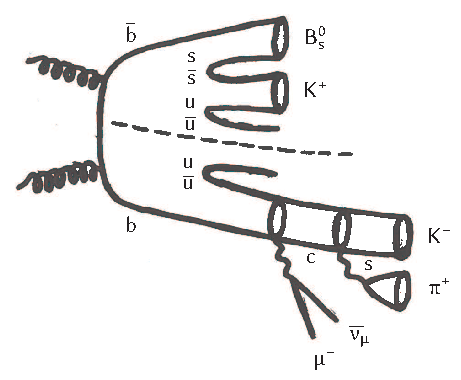
\includegraphics{graphics/intro/tikz/tagging}
  \caption{Production and decay mechanisms exploited by flavour-tagging algorithms.
           Same-side tagging determines the flavour of the $\Bs$ or $\Bsbar$ meson from the charge of the kaon that is produced close to it
           (top half of the figure).
           Opposite-side tagging determines the flavour from the charges of the decay products of the ``opposite'' b or $\qbar[b]$ quark in
           the event
           (bottom half of the figure).}
  \label{fig:tagging}
\end{figure}

The charge of the beauty quark on the ``opposite side of the event'' can be determined from the charges of the electron, muon, or kaon in
the decay of the hadron it formed. This procedure is termed \emph{opposite-side tagging} and is described in
reference~\cite{LHCb-PAPER-2011-027}.

The efficiency of opposite-side tagging is limited. The required charged particles are produced in many, but not all beauty decays. In
addition, the decay products may not be detectable by the LHCb detector. There is also a probability that the determined flavour is wrong.
A neutral beauty meson may convert into its antiparticle before it decays, which gives the opposite tag. A background of charged particles
from elsewhere in the event gives additional wrong tags. The resulting effective fraction of $\Bs$ mesons with a correct opposite-side tag
in the \BstoJpsiKK{} measurement is 2.6\% (see Section~\ref{sec:exp_tagging}).

When combined with an (anti)up quark, the remaining quark from the s$\qbar[s]$ pair forms a charged kaon. In \emph{same-side kaon tagging}
the flavour of the $\Bs$ meson is estimated by determination of the charges of kaons that are close to it in momentum
space~\cite{LHCb-CONF-2012-033}. This procedure is limited by other possibilities for fragmentation and hadronization of the strange quark
and by detection of the correct kaon. The effective fraction of $\Bs$ mesons with a correct same-side tag is 1.3\% in the \BstoJpsiKK{}
measurement.


%%%%%%%%%%%%%%%%%%%%%%%%%%%%%%%%%%%%%%%%%%%%%%%%%%%%%%%%%%%%%%%%%%%%%%%%
\subsection{\texorpdfstring{\BstoJpsiKK}{Bs0->J/psi K+K-} Decays in LHCb}
\label{subsec:intro_LHCb_Jpsiphi}
%%%%%%%%%%%%%%%%%%%%%%%%%%%%%%%%%%%%%%%%%%%%%%%%%%%%%%%%%%%%%%%%%%%%%%%%

LHCb is one of the four large experiments that analyse the particles produced by LHC collisions. The LHCb detector measures particle
trajectories in the ``forward'' direction, that is, along the direction of one of the proton beams. Particles produced with momenta at
angles between typically 1 and 15 degrees from the beam direction can be detected. Although this \emph{acceptance region} covers only a
small part of possible particle directions, it contains roughly a quarter of all produced beauty quarks. This makes the LHCb design
efficient for studies of hadrons containing beauty quarks.

The particles that are produced in an LHC collision get a momentum from the boost introduced by asymmetric parton momenta, but also from
the centre-of-mass energy that is available in the parton interaction. $\Bs$ mesons that are selected for the analysis of \BstoJpsiKK{}
decays have an average momentum of the order of a hundred \GeVc{} (see Figure~\ref{fig:introHists_BMomentum}). With the 5.4\unitsp\GeV{}
$\Bs$-meson mass~\cite{PDG}, this gives an average Lorentz factor of about 20.

The $\Bs$ meson has a relatively large mean lifetime of about 1.5\unitsp{}ps \cite{Amhis:2012bh}. As a result of the significant lifetime
and boost, $\Bs$ mesons cover a typical distance of several millimetres before they decay. The measurement of this \emph{flight distance}
is used to infer the decay time. It is determined by reconstructing the positions of the points of production and decay. The measured
distribution for $\Bs$ mesons that are used in the \BstoJpsiKK{} measurement is shown in Figure~\ref{fig:introHists_flightDist}.

\begin{figure}[tbhp]
  \centering
  \begin{subfigure}{0.497\textwidth}
    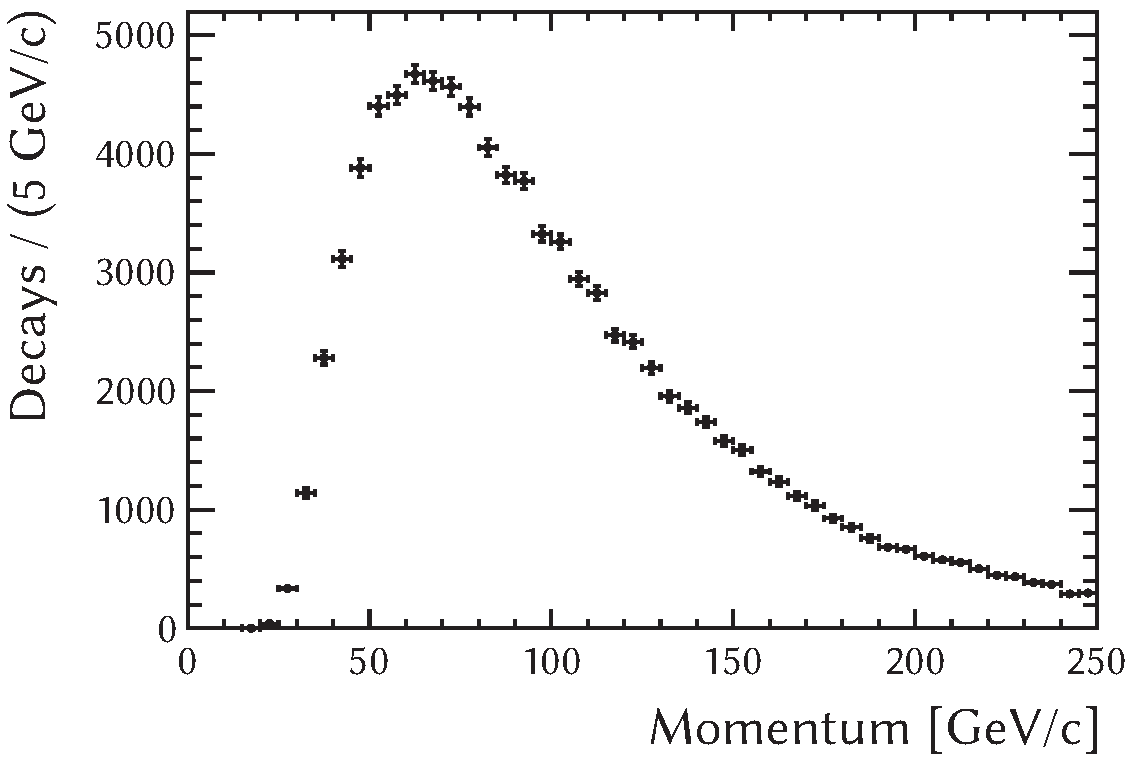
\includegraphics[width=\textwidth]{graphics/intro/BMomentum}
    \caption{}
    \label{fig:introHists_BMomentum}
  \end{subfigure}%
  \hfill%
  \begin{subfigure}{0.497\textwidth}
    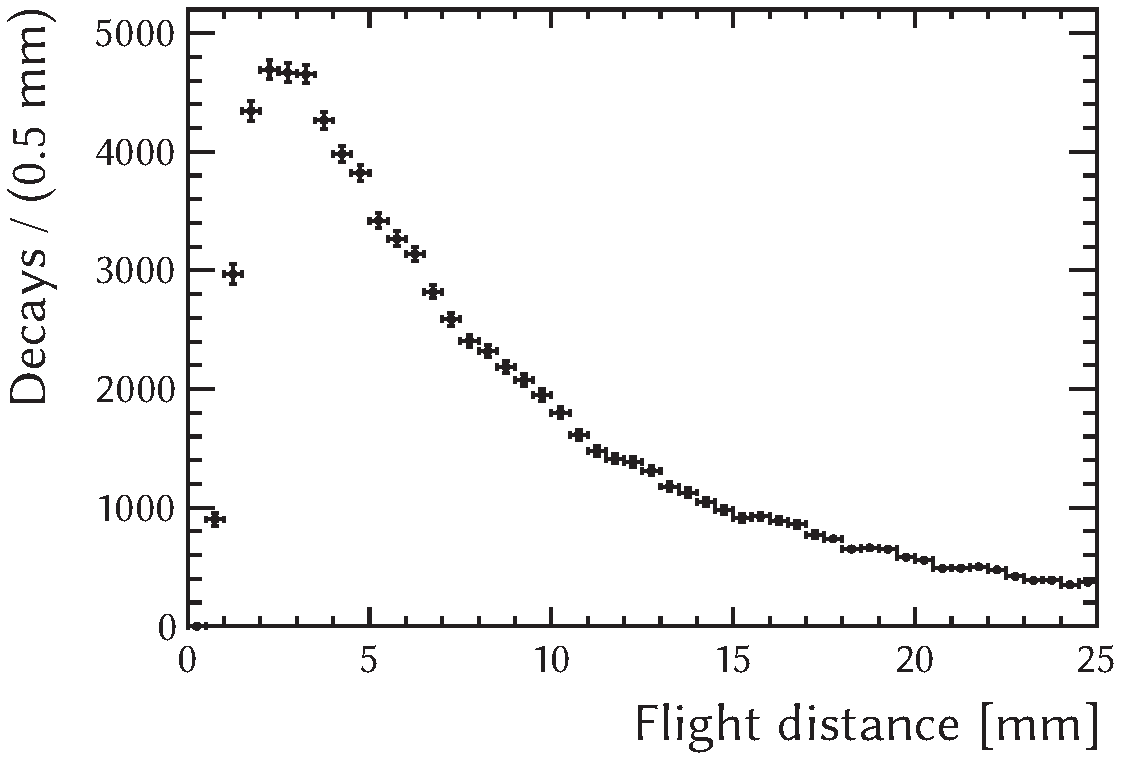
\includegraphics[width=\textwidth]{graphics/intro/flightDist}
    \caption{}
    \label{fig:introHists_flightDist}
  \end{subfigure}
  \caption{Histograms of (a) the reconstructed momenta and (b) the flight distance of $\Bs$ mesons in the \BstoJpsiKK{} measurement.}
  \label{fig:introHists}
\end{figure}

Since LHC bunches have a finite size and the positions of the colliding protons in their respective bunches are not known a priori, the
interaction point has to be measured for each collision. This is done by measuring the trajectories of produced particles and extrapolating
them to the point of their common origin. This point is termed the \emph{primary vertex}. The \emph{secondary vertex} is the point where
the $\Bs$ decayed, which is measured with only the trajectories of the four decay $\Bs$ products.

Figure~\ref{fig:vertices} schematically shows the vertices in the \BstoJpsiKK{} decay. The vertices are depicted by ellipsoids with a size
that represents the uncertainty in the vertex position. The resolution on the vertex position is better for the primary vertex than for the
secondary vertex, because a larger number of particles is used for the reconstruction of the former.

The secondary vertex is constructed from the $\mumu$ vertex and the $\KK$ vertex, where the former dominates because of a better
resolution. This difference is caused by the fact that only $\KK$ invariant masses in between 0.99 and 1.05~\GeV{} are selected, which is
just above the threshold of twice the kaon mass. As a result, the opening angle between the $\Kp$ and $\Km$ trajectories is small, which
gives the measurement of the point of common origin a large uncertainty.

\begin{figure}[ptb]
  \centering
  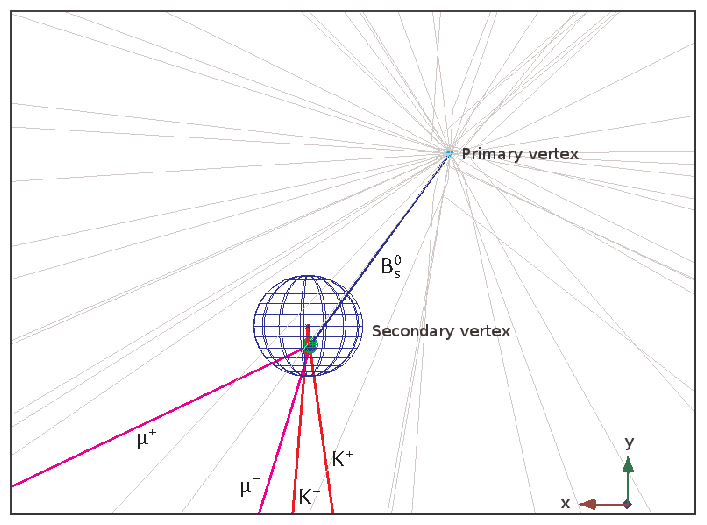
\includegraphics{graphics/intro/tikz/vertices}
  \caption{Vertices in a \BstoJpsiKK{} decay \cite{vanEijk:2012}.
           The vertices are indicated by ellipsoids with a size that represents the uncertainty in the vertex position.
           The primary vertex is indicated by the cyan ellipsoid, the $\mumu$ vertex with the small green ellipsoid
           and the $\KK$ vertex with the large blue ellipsoid.
           The secondary vertex is the combination of the $\mumu$ and $\KK$ vertices.}
  \label{fig:vertices}
\end{figure}

The decay time can be calculated from the flight distance if also the $\Bs$ momentum is known:
\begin{equation}
  \label{eq:decayTime}
  t = \frac{1}{\gamma(v)}\,\frac{d}{v} = \frac{m d}{\gamma(v) m v} = \frac{m d}{|\vec{p}|} \ \ ,
\end{equation}
where $t$ is the decay time in the rest system of the $\Bs$, $d$ the flight distance, $v$ the $\Bs$ velocity, $\gamma$ the
corresponding Lorentz factor, $\vec{p}$ the momentum, and $m$ the $\Bs$ mass. The momentum is reconstructed as a vector sum of the
decay-product momenta, which are also required to calculate the decay angles. Momenta of charged particles are inferred from the curvature
of their tracks in the magnetic field of the detector.

The $\Bs$ momentum and flight distance are estimated by combining information from measured particle momenta and extrapolated
positions~\cite{Hulsbergen:2005pu}. Uncertainties in the measurements are propagated and ultimately lead to an uncertainty in the estimated
decay time. This decay-time resolution is estimated for each $\Bs$ decay and taken into account in the analysis (see
Sections~\ref{sec:exp_time} and \ref{subsec:ana_model_timeRes}). The effective resolution is about 0.05\unitsp{}ps. This suffices to
resolve the oscillations in the \BstoJpsiKK{} decay-time distribution, which have a period of 2π/$\Dms$\textapprox0.35\unitsp{}ps.

Before the vertex positions and momenta can be determined, the four particles from a \BstoJpsiKK{} decay have to be selected from all
particles that are produced in an LHC event. Since the particle multiplicity is high, there is a significant probability to select four
particles that do not originate from a $\Bs$ decay.

Combinations of four particles that are considered for analysis are called \emph{decay candidates}. Candidates can either be real
\BstoJpsiKK{} decays (\emph{signal}) or combinations that fake the decay signature (\emph{background}). Distributions of decay time and
decay angles for background events are subtracted from the measured distributions to obtain the net signal contribution (see
Section~\ref{sec:ana_bkg}).

There are several categories of background decay candidates. Most background is \emph{combinatorial}, which means that candidates are
formed from random combinations of four particles. Often all four particles originate directly from a primary vertex. This combinatorial
background is called \emph{prompt}. For non-prompt candidates some of the particles originate from a secondary vertex in the decay of a
long-lived particle, for example a beauty hadron. Since the $\mumu$ vertex has a relatively small uncertainty in comparison with the $\KK$
vertex, this often involves a $\Jpsi\to\mumu$ decay combined with kaons from the primary vertex.

Another category is \emph{misidentified background}, which comprises decays where one or more particles have been incorrectly identified.
The two misidentified backgrounds that are taken into account in the \BstoJpsiKK{} measurement are \BdtoJpsiKstKpi{} and \LbtoJpsipK. In
the $\Bd$ decay the pion is misidentified as a kaon and in the $\Lb$ decay the proton as a kaon.

There are different stages of event and decay-candidate selection. Each stage is optimized to find signal decays with high efficiency and
at the same time keep the background at a manageable level. The first three selection stages are \emph{triggers} \cite{LHCb-DP-2012-004},
which are designed to select events of interest \emph{online}, before detector data are stored for further analysis. Two \emph{offline}
stages select decay candidates in the stored events.

The first trigger is called \emph{Level 0} (L0). It is implemented in the detector hardware and designed to bring the rate of incoming
events down to less than 1\unitsp{}MHz. In proton collisions that create beauty hadrons, particles are created in all directions in the
centre-of-mass frame of the parton interaction. As a result, particles in these collisions typically have significant momentum components
in the direction transverse to the proton beams. This is used by the L0 trigger, which selects only events that contain particles with a
minimum transverse momentum.

Events that are selected by L0 are processed by the \emph{High Level Trigger} (HLT). This trigger is implemented in software and consists
of two stages: HLT1 and HLT2. In the first stage a minimal reconstruction of particle trajectories and vertices is performed. For the
\BstoJpsimumuKK{} measurement, events are selected if they contain the signatures of the muons in this decay.

HLT1 selects roughly 40\unitsp{}kHz of events, which are subsequently processed by HLT2. At this stage a more complete particle
reconstruction is performed. Events are selected for the \BstoJpsiKK{} measurement if they contain $\mumu$ pairs that are compatible with a
$\Jpsi$ decay at a significant distance from a primary vertex. About 3\unitsp{}kHz of events is stored for all LHCb measurements.

The first stage of the offline selection fully reconstructs the particle trajectories and vertices in the remaining events and selects
combinations of muon and kaon pairs that form \BstoJpsiKK{} candidates. A set of loose selection criteria is applied to filter out
part of the background, which reduces the number of remaining candidates to a manageable level. This procedure is termed \emph{stripping}.

Stripping yields about one million \BstoJpsiKK{} decay candidates for 2011 and 2012. A second set of stricter offline selection criteria is
optimized to find the best compromise between selecting as many signal and as few background candidates as possible. About 230 thousand
candidates are used for further analysis, of which roughly 40\% is signal (see Sections~\ref{sec:exp_selBkg} and \ref{sec:ana_bkg}).

The total set of selection requirements for particles and decay candidates removes background, but also a significant part of the signal.
%This can be seen in the flight-distance distribution of Figure~\ref{fig:introHists_flightDist}. The original decay-time distribution has
%approximately an exponential shape. Since the decay time and $\Bs$ momentum are uncorrelated, also an exponential shape is expected for the
%flight-distance distribution. The lack of entries at small flight distance is a result of the selection inefficiency.
Since the efficiency of the selection depends on the decay time and the decay angles, the observed distributions of these variables do not
directly reflect the underlying true distributions. This effect has to be taken into account in the model of the decay (see
Sections~\ref{sec:exp_time}, \ref{sec:exp_angles} and \ref{sec:ana_model}).


%%%%%%%%%%%%%%%%%%%%%%%%%%%%%%%%%%
\subsection{The LHCb Detector}
\label{subsec:intro_LHCb_detector}
%%%%%%%%%%%%%%%%%%%%%%%%%%%%%%%%%%

\begin{figure}[ptb]
  \centering
  \begin{subfigure}{0.78\textwidth}
    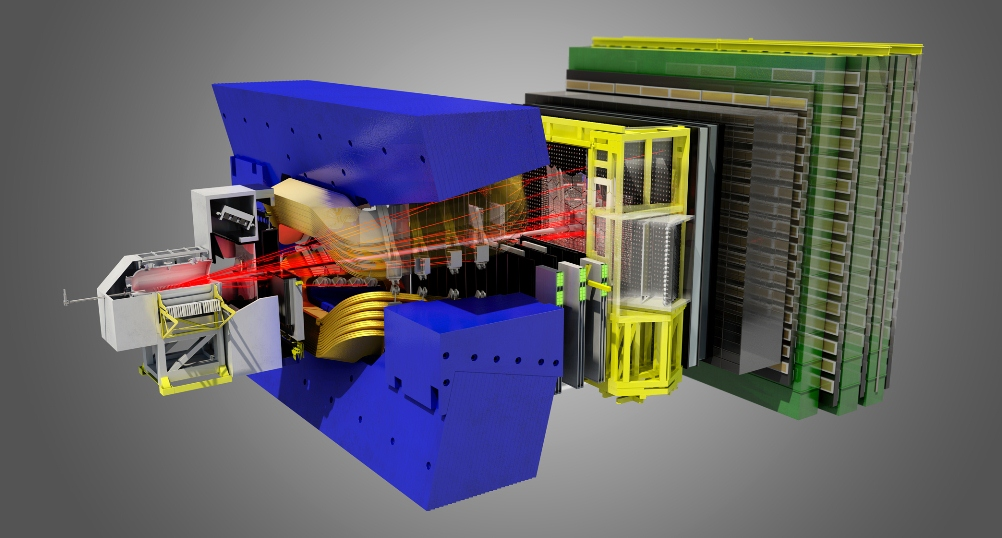
\includegraphics[width=\textwidth]{graphics/intro/detector_3D.jpg}
    \caption{}
    \label{fig:LHCb_3D}
  \end{subfigure}

  \vspace*{0.03\textwidth}
  \begin{subfigure}{\textwidth}
    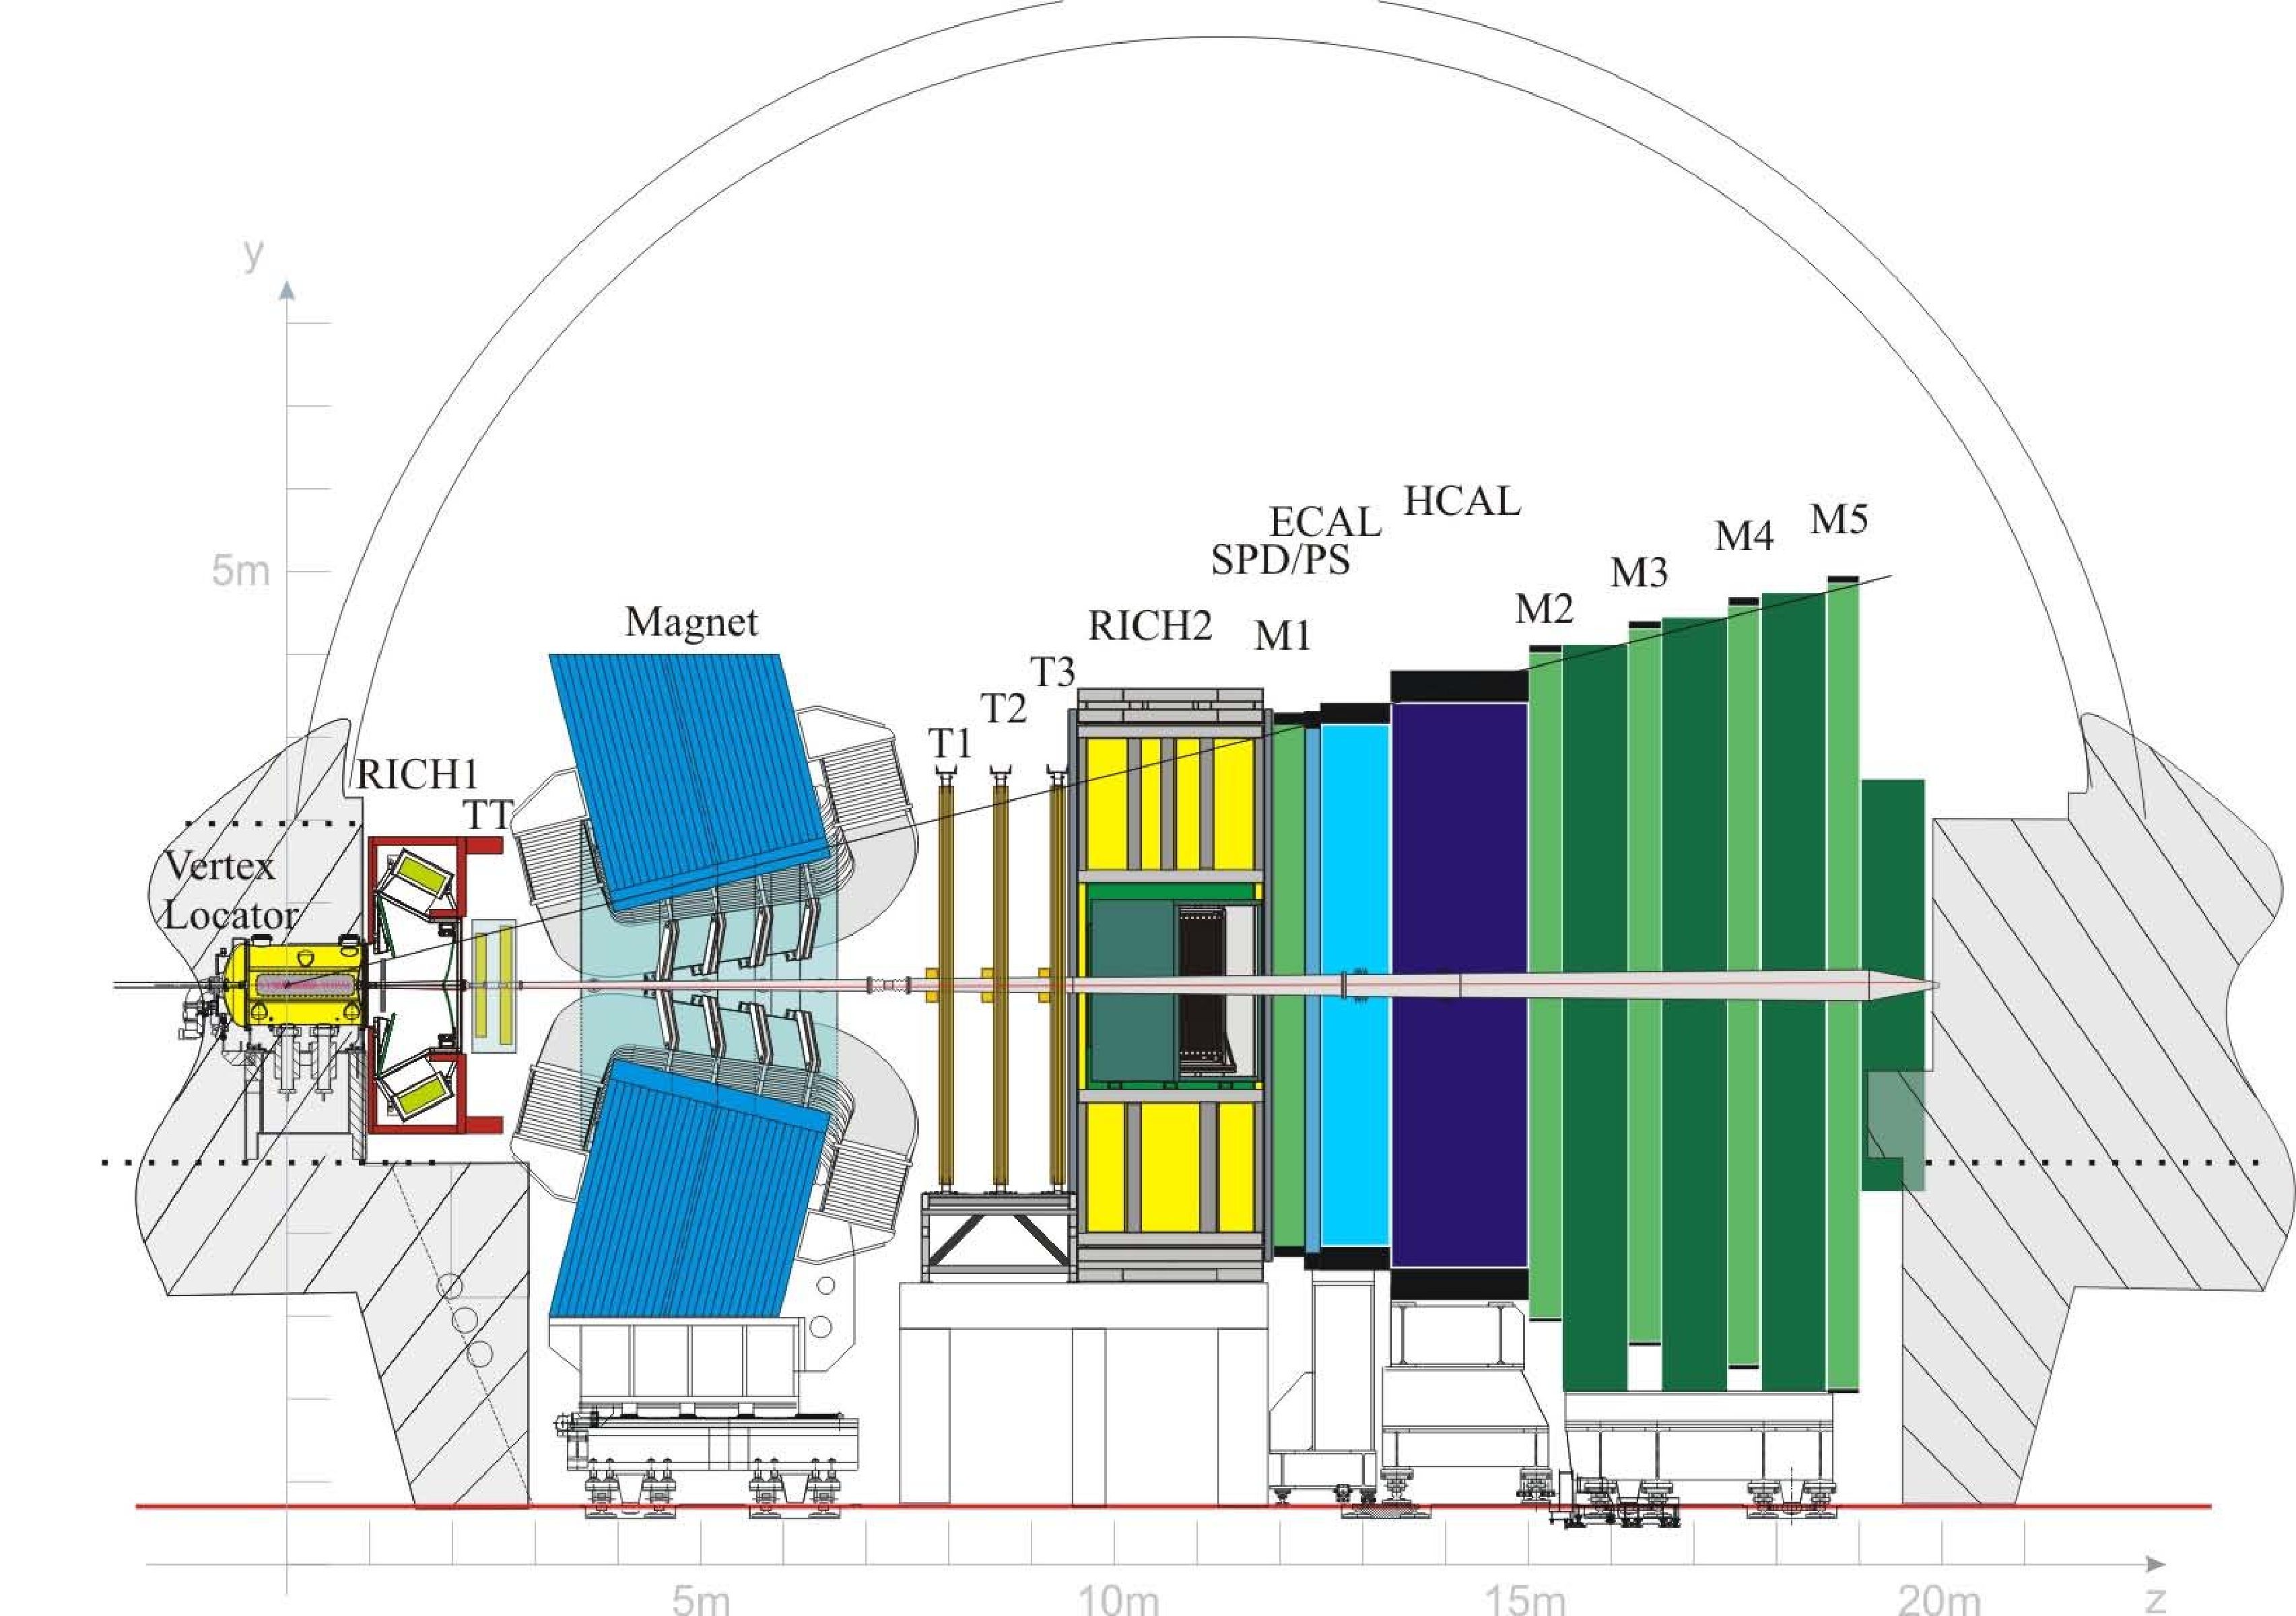
\includegraphics[width=\textwidth]{graphics/intro/detector_cross}
    \caption{}
    \label{fig:LHCb_cross}
  \end{subfigure}

  \caption{Schematic views of the LHCb detector.
           (a) Three-dimensional view, where particles from the proton--proton collision are depicted by red lines.
           (b) Cross sectional view of the various subdetectors, which are discussed in the text.}
  \label{fig:LHCb}
\end{figure}

The LHCb detector was mainly built to measure beauty- and strange-hadron decays into particles with an electric charge. It is capable of
measuring charged-particle trajectories and the locations of primary and secondary vertices with a precision that is good enough to resolve
oscillations in decay-time distributions with a frequency $\Dms$\textapprox18\unitsp{}ps. Another important feature of the detector is its
ability to identify different types of particles.

The detector is described in detail in reference~\cite{Alves:2008zz}. A schematic view is shown in Figure~\ref{fig:LHCb}. The subdetectors
were built around the LHC beams, which come in from the left and right. The interaction point is contained within the subdetector labelled
``Vertex Locator'' on the left of Figure~\ref{fig:LHCb_cross}. Particles that are produced within the LHCb acceptance region traverse the
various subdetectors from the left to the right. This is indicated by the red lines in Figure~\ref{fig:LHCb_3D}.

A magnetic field with an integrated strength of 4\unitsp{}Tm is produced by a dipole magnet between approximately 3 and 8\unitsp{}m from
the interaction point. The saddle-shaped coils of the magnet are surrounded by the magnet yoke, which is indicated by the blue block in
Figure~\ref{fig:LHCb}. The magnetic field is pointing either upwards or downwards, bending charged-particle trajectories in the horizontal
plane. During the two years of LHC running, the direction of the magnetic field was reversed several times to control systematic
uncertainties related to the measurement of particle trajectories.

Trajectories of charged particles are reconstructed by measurement of the positions at which the particles traverse the various
\emph{tracking detectors} of LHCb. These measurements are all based on electromagnetic interactions of the particle with detector material.
The signal from a particle interaction with a unit of sensitive detector material is called a \emph{hit}. The collection of hits that
represent the trajectory of a particle is a \emph{track}.

The LHCb tracking system consists of four components. The \emph{Vertex Locator} (\velo) and the \emph{Tracker Turicensis} (TT)
before the magnet and the \emph{Inner Tracker} (IT) and \emph{Outer Tracker} (OT) behind the magnet. Together, the IT and OT form the
three tracking stations labelled by ``T1'', ``T2'', and ``T3'' in Figure~\ref{fig:LHCb_cross}. The inner region of roughly
0.5\unitsp{}m\textsuperscript{2} around the proton beams is covered by the IT and the region up to approximately 3\unitsp{}m from the beams
by the OT.

Hit information from all tracking detectors is combined to build tracks. The momentum of a particle can be inferred from the radius of
curvature of the track in the magnetic field, given the charge of the particle. Since most charged particles that live long enough to reach
the detector are electrons, muons, pions, kaons, and protons, a unit charge can be assumed. The sign of the charge is determined from the
direction of the track curvature.

The performance of the tracking system is shown in Figures~\ref{fig:detPerf_momRes} and \ref{fig:detPerf_massRes}. The former figure shows
the relative resolution of the momentum measurement for muon tracks in $\Jpsi\to\mumu$ decays, which varies from roughly 0.5\% to 1.1\% as
a function of momentum. The resulting resolution of the dimuon invariant-mass measurement is shown in the latter figure. The relative mass
resolution is about 0.5\% up to 10\unitsp\GeV, but increases to 1.9\% at the $\Zz$ mass.
\begin{figure}[ptb]
  \begin{subfigure}{0.49\textwidth}
    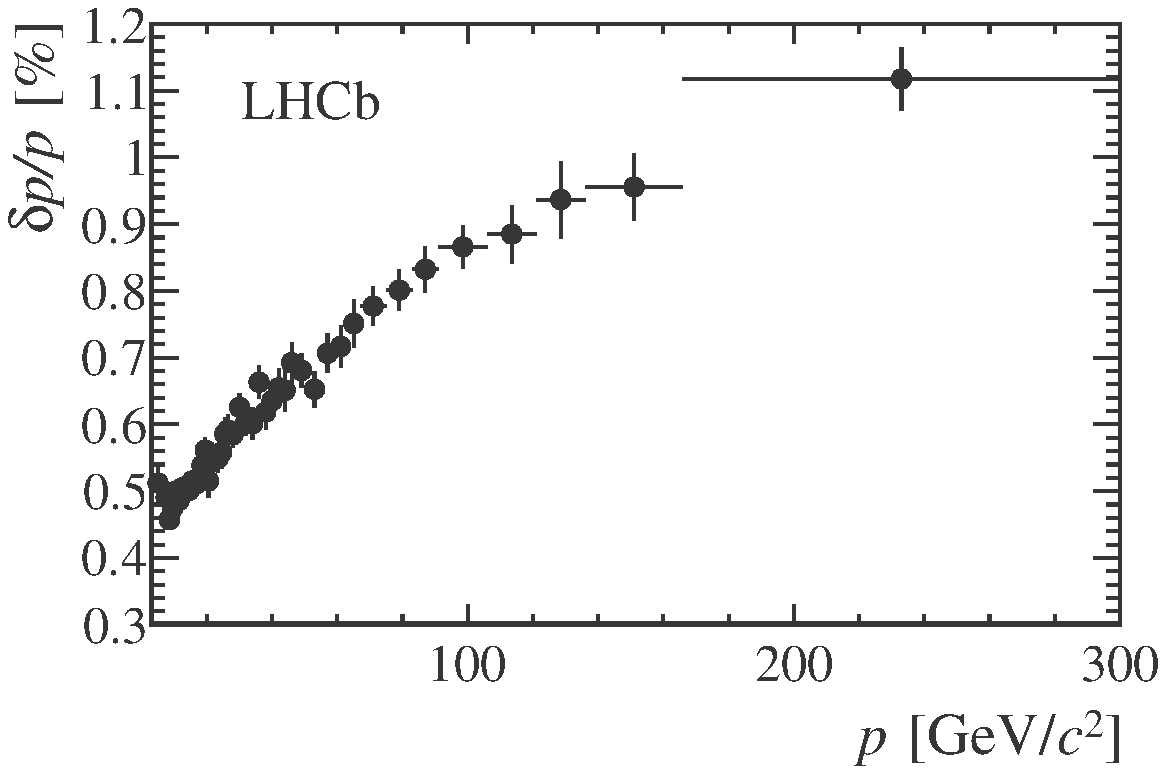
\includegraphics[width=\textwidth]{graphics/intro/dppVsp-crop-cmyk}
    \caption{}
    \label{fig:detPerf_momRes}
  \end{subfigure}%
  \hfill%
  \begin{subfigure}{0.49\textwidth}
    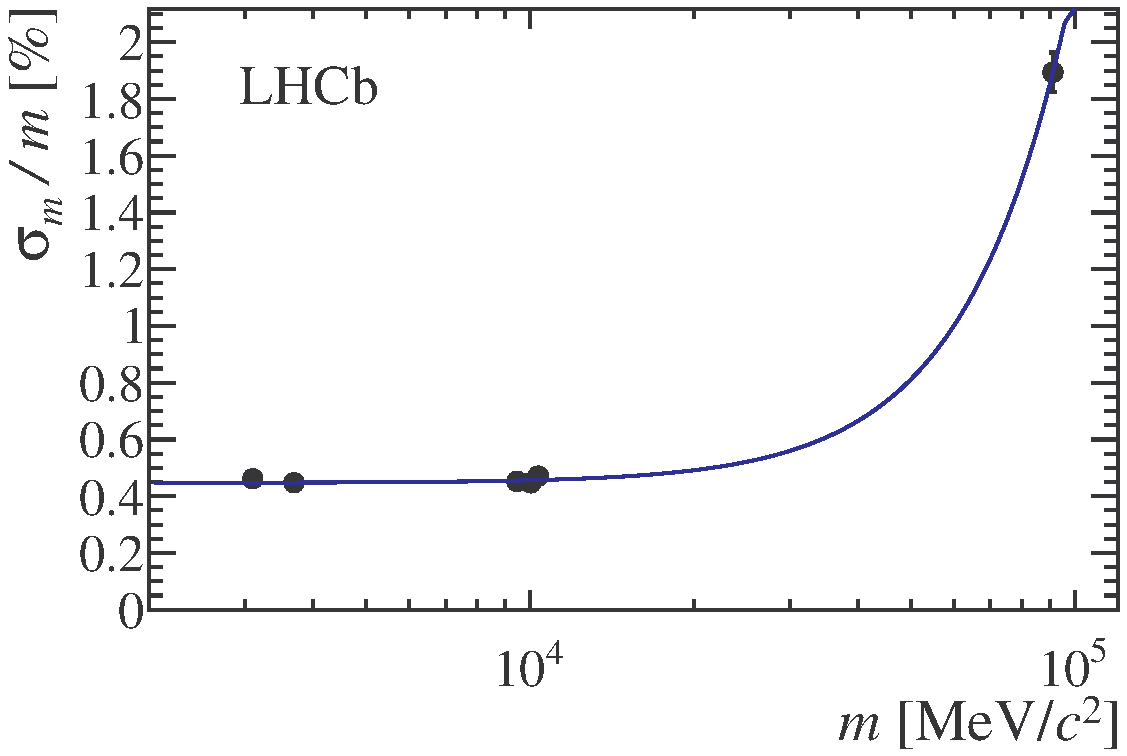
\includegraphics[width=\textwidth]{graphics/intro/relResolutionVsMass-crop-cmyk}
    \caption{}
    \label{fig:detPerf_massRes}
  \end{subfigure} \\

  \vspace*{0.01\textwidth}

  \begin{subfigure}{0.49\textwidth}
    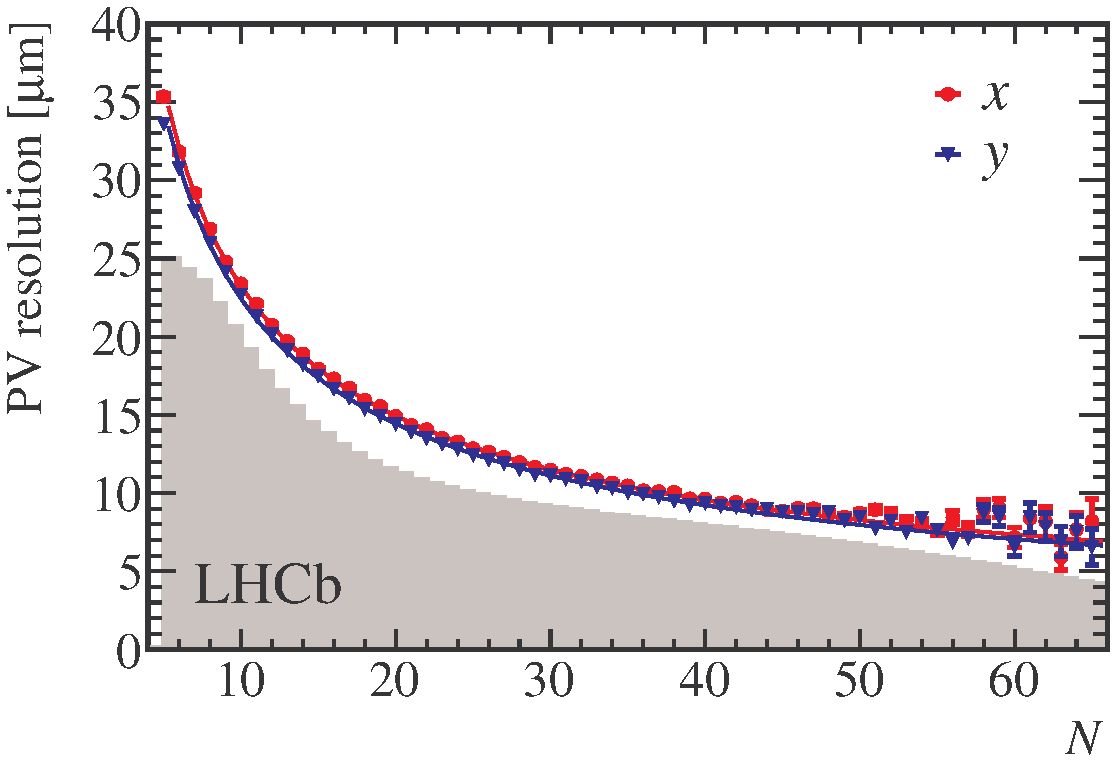
\includegraphics[width=\textwidth]{graphics/intro/DataResXY_1PV_2012-crop-cmyk}
    \caption{}
    \label{fig:detPerf_vertRes}
  \end{subfigure}%
  \hfill%
  \begin{subfigure}{0.49\textwidth}
    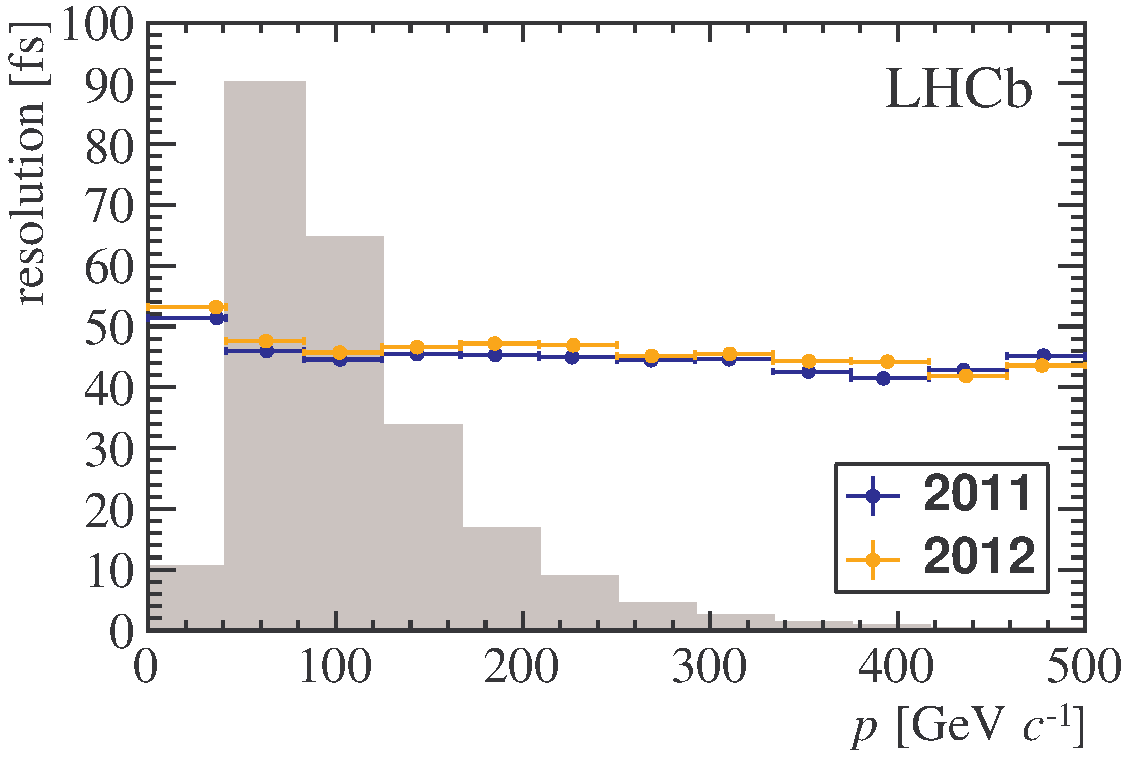
\includegraphics[width=\textwidth]{graphics/intro/decaytimeresoVsMomentumJPsiPhi-crop-cmyk}
    \caption{}
    \label{fig:detPerf_timeRes}
  \end{subfigure}

  \caption{Performance of the LHCb detector.
           (a) Relative momentum resolution as a function of momentum for muon tracks in $\Jpsi\to\mumu$ events.
           (b) Relative $\mumu$ invariant-mass resolution as a function of mass,
               measured for the $\Jpsi$, $\psitwoS$, $\upsS[1]$, $\upsS[2]$, $\upsS[3]$, and $\Zz$ resonances.
           (c) Primary vertex resolution as a function of the number of tracks in the vertex,
               separately for the two directions in the plane transverse to the beam direction.
           (d) Decay-time resolution of prompt \BstomumuKK{} background as a function of the combined $\mumu\,\KK$ momentum,
               separately for 2011 and 2012.}
  \label{fig:detPerf}
\end{figure}

Vertices are reconstructed by extrapolating tracks to the point where they are closest together. The most precise information on vertex
locations comes from the \velo, which detects particles very close to the interaction point down to a radius of 8\unitsp{}mm
around the beams.

Figure~\ref{fig:detPerf_vertRes} shows the resolution of primary vertices in LHCb as a function of the number of tracks originating from
the vertex. A minimum of five tracks is required, where the resolution is about 35\unitsp\micron. The resolution improves with the number
of tracks to less than 10\unitsp\micron{} for more than 40 tracks.

Since only four tracks originate from the secondary vertex, its resolution dominates the uncertainty of the decay-time measurement. For
\BstomumuKK{} events the decay-time resolution is measured with prompt background, for which the true decay time is equal to zero (see
Section~\ref{sec:exp_time}). The resulting resolution as a function of $\mumu\,\KK$ momentum is shown in Figure~\ref{fig:detPerf_timeRes}.
Its value varies between roughly 0.04\unitsp{}ps and 0.05\unitsp{}ps.

Particles are identified with other subsystems. Electrons produce signals in the \emph{Scintillator Pad Detector} (SPD), \emph{Preshower
detector} (PS) and the \emph{Electromagnetic Calorimeter} (\ecal). The electron energy is absorbed by these detectors and no signal is
produced in the \emph{Hadronic Calorimeter} (\hcal). Pions, kaons, and protons predominantly lose energy in the \hcal{} and less in the
\ecal. Energy measurements from the calorimeters are also used in the L0 trigger to select events with high-energy particles in the
transverse direction.

Muons do not lose significant energy in the \hcal, make it through the calorimeters, and produce hits in the four \emph{muon stations}
behind the \hcal{} (M2--M5 in Figure~\ref{fig:LHCb_cross}). These features distinguish muons from hadrons. The \emph{Muon System} is
completed by the station M1 before the calorimeters to provide an optimal momentum estimate for muons.

Two \emph{Ring Imaging Cherenkov} (\rich) detectors are used to distinguish the different charged hadrons. The first \rich{} detector
(\rich1) is located between the \velo{} and the magnet and the other (\rich2) behind the IT/OT. These detectors determine the velocities of
charged particles by measuring the angle at which Cherenkov light is emitted when the particle traverses the \rich{} radiator materials.
Combined with the momentum measurement this gives an estimate of the particle mass to distinguish between pions, kaons, and protons.

Figure~\ref{fig:event} shows the information from different subdetectors for an event that contains a \BstoJpsiKK{} decay candidate. The
coloured lines show reconstructed tracks. Three tracks are combined with hits in the muons stations and represent particles that have been
identified as muons.
\begin{figure}[ptb]
  \centering
  \begin{tikzpicture}
    \node[anchor=south]{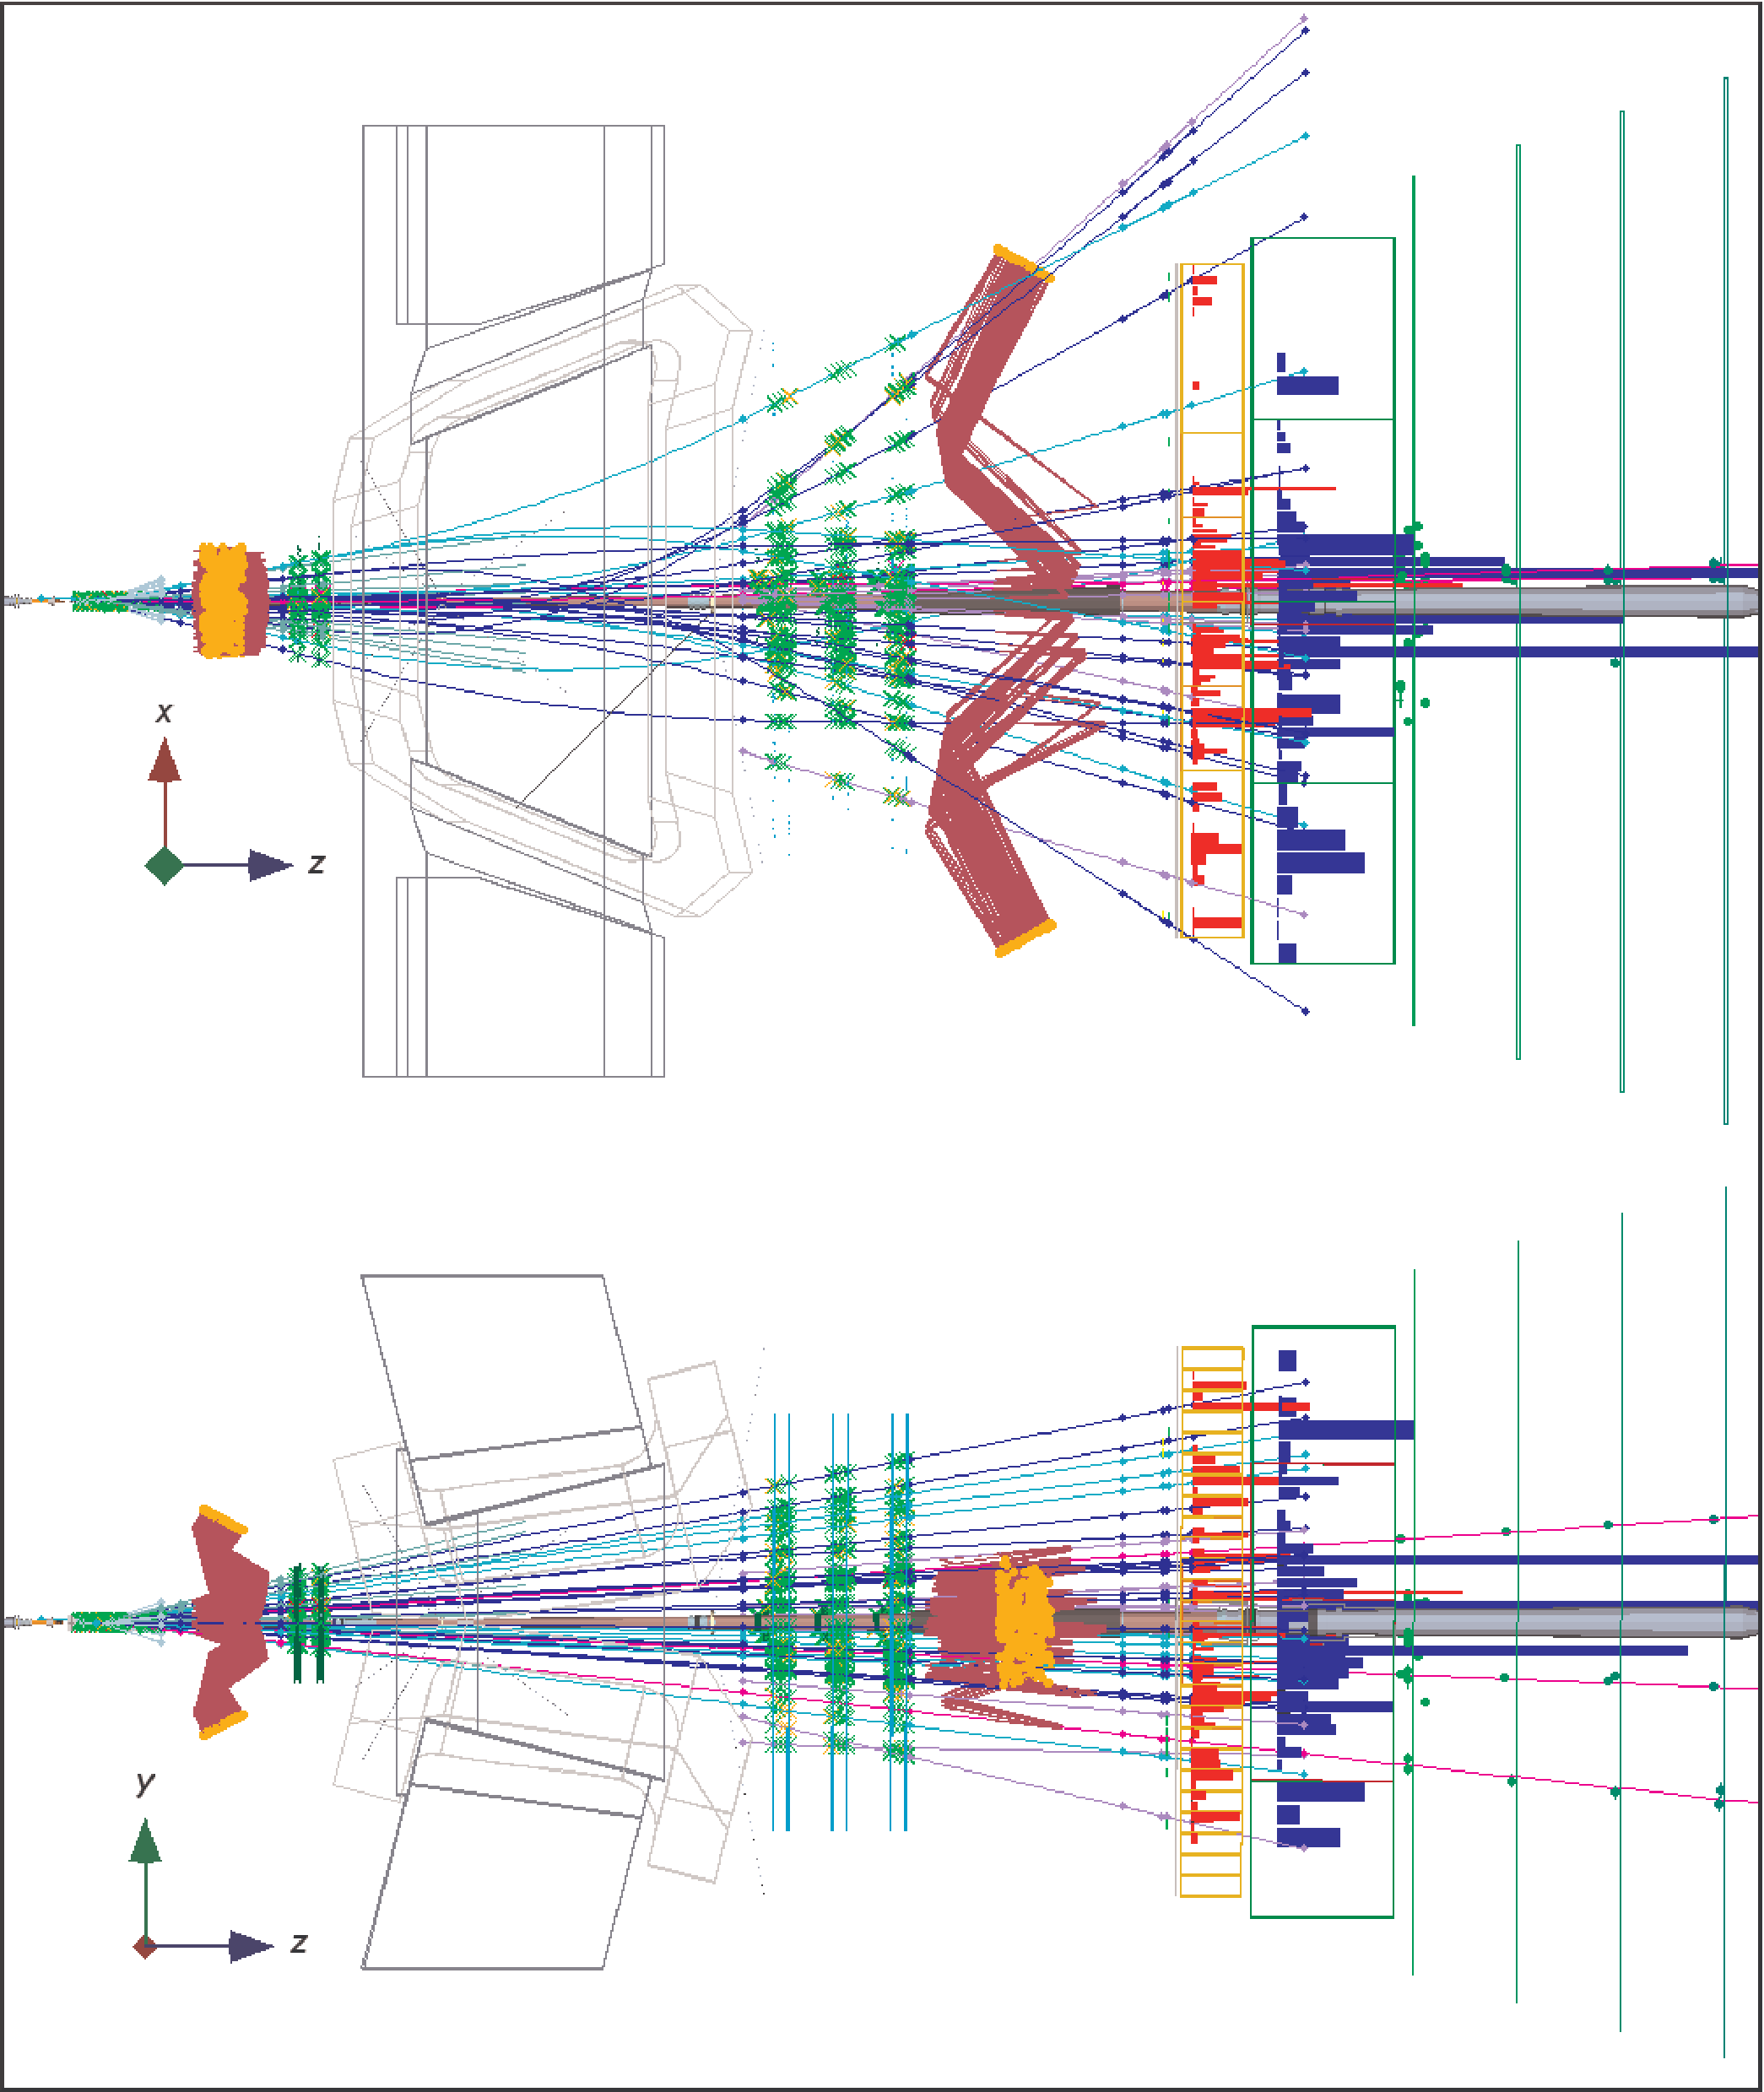
\includegraphics[width=0.95\textwidth]{graphics/intro/eventdisplay_CMYK}};
    \node at ( 0., 6.7 )  {\textbf{(a)}};
    \node at ( 0., 0.7 )  {\textbf{(b)}};
  \end{tikzpicture}
  \caption{Reconstructed particle trajectories in the LHCb detector for an event with a \BstoJpsiKK{} decay candidate \cite{vanEijk:2012}:
           (a) a view from the top and (b) a view from the side, equivalent to Figure~\ref{fig:LHCb}.
           Particle tracks are shown by the coloured lines. The green crosses indicate hits in the tracking detectors and the red and blue
           bars energy deposits in the calorimeters. Hits in the muon stations are represented by green dots. Cherenkov photons in the
           \rich{} detectors are shown by the purple lines and orange hits.}
  \label{fig:event}
\end{figure}

